\begin{appendix}
%\appendixpage
\noappendicestocpagenum
\addappheadtotoc
\chapter{Decription of the training workflow}
\label{appendix:training_workflow}
Below one can find description of the complete procedure for training the system classifiers.
\begin{enumerate}
\item Get CERMINE source code. It is available publicly on the Web.
\lstset{language=bash}
\begin{lstlisting}
git clone https://github.com/pszostek/CERMINE.git
cd CERMINE
\end{lstlisting}
\item Build CERMINE using maven by running the following Bash script from the CERMINE main directory. It assumes that the \verb+PATH+ variable contains a path to \verb+mvn+.
\begin{lstlisting}
#!/usr/bin/env bash
curdir=$PWD
cd cermine-impl && mvn package -DskipTests && mvn assembly:single && cd $curdir
cd cermine-tools && mvn package -DskipTests && mvn assembly:single && cd $curdir
\end{lstlisting}
\item Create files with samples for the classifiers using GROTOAP2. To this end, one need to run the following script. Note that the \verb+GROTOAP2_PATH+ variable has to point to a directory containing cxml files from the dataset.
\begin{lstlisting}
#!/usr/bin/env bash
BASE=$(dirname $(pwd))
java -Djava.util.Arrays.useLegacyMergeSort=true -cp \
    $BASE/cermine-tools/target/cermine-tools-1.2-SNAPSHOT-jar-with-dependencies.jar:\
    $BASE/cermine-impl/target/cermine-impl-1.2-SNAPSHOT-jar-with-dependencies.jar:\
    $BASE/cermine-impl/target/cermine-impl-1.2-SNAPSHOT.jar pl.edu.icm.cermine.libsvm.LibSVMExporter $GROTOAP2_PATH
\end{lstlisting}
\item Scale down the samples' feature values so that those with relatively huge absolute values do not dominate those with smaller values. This is a step recommended in \cite{Chih-WeiHsu2010}. It can be done by using the svm-scale tool from \verb+libsvm+ package.
\begin{lstlisting}
svm-scale -l -1 -u 1 -s range1 meta_GROTOAP2 > meta_GROTOAP2.scale
svm-scale -l -1 -u 1 -s range1 initial_GROTOAP2 > initial_GROTOAP2.scale
\end{lstlisting}
\item Find the best parameters for the classifiers using \verb+grid.py+ from the \verb+libsvm+ package. The below script can facilitate iterating over different kernel types. One need to pick the classifier with the lowest error rate.
\begin{lstlisting}
#!/usr/bin/env bash
for classifier in meta initial; do
        for kernel in $(seq 0 3); do
                printf "kernel=$kernel: "
                if [ $kernel -eq 1 ]; then
                        degree=" -d 4 "
                else
                        degree=""
                fi
                /root/grid.py -t $kernel -gnuplot /usr/local/bin/gnuplot -svmtrain /root/libsvm-3.18/svm-train $degree ${classifier}_GROTOAP.dat.scale
        done
done
\end{lstlisting}
\item Using the optimal parameters, train the classifiers and save them to files. The below command has to be run from the main CERMINE directory. The variables \verb+KERNEL_I+, \verb+G_I+, \verb+C_I+ and \verb+D_I+ indicate respectively the kernel type, the $\gamma$ parameter, the $C$ parameter and possibly polynomial degree of the initial zone classification kernel. Variables \verb+KERNEL_M+, \verb+G_M+, \verb+C_M+ and \verb+D_M+ indicate respectively the kernel type, the $\gamma$ parameter, the $C$ parameter and possibly polynomial degree of the metadata classification kernel.
\begin{lstlisting}
#!/usr/bin/env bash
java -Djava.util.Arrays.useLegacyMergeSort=true -cp \
    ./cermine-tools/target/cermine-tools-1.2-SNAPSHOT-jar-with-dependencies.jar\
    ./cermine-impl/target/cermine-impl-1.2-SNAPSHOT-jar-with-dependencies.jar\
    ./cermine-impl/target/cermine-impl-1.2-SNAPSHOT.jar\
    pl.edu.icm.cermine.tools.classification.svm.SVMInitalBuilder -input\
        initial_GROTOAP2.dat.scale -output CERMINE_initial_classifier\
        -kernel $KERNEL_I -g $G_I -C $C_I [-degree $D_I]

java -Djava.util.Arrays.useLegacyMergeSort=true -cp \
    ./cermine-tools/target/cermine-tools-1.2-SNAPSHOT-jar-with-dependencies.jar\
    ./cermine-impl/target/cermine-impl-1.2-SNAPSHOT-jar-with-dependencies.jar\
    ./cermine-impl/target/cermine-impl-1.2-SNAPSHOT.jar\
    pl.edu.icm.cermine.tools.classification.svm.SVMMetadataBuilder -input\
        meta_GROTOAP2.dat.scale -output CERMINE_meta_classifier\
        -kernel $KERNEL_M -g $G_M -C $C_M [-degree $D_M]
\end{lstlisting}
\item Parameters from the previous step can be used to evaluate the classifier. CERMINE contains full classes that perform n-fold cross-validation. To obtain full validation reports, one need to run the commands that follow.
\begin{lstlisting}
#!/usr/bin/env bash
java -Djava.util.Arrays.useLegacyMergeSort=true -cp \
    ./cermine-tools/target/cermine-tools-1.2-SNAPSHOT-jar-with-dependencies.jar\
    ./cermine-impl/target/cermine-impl-1.2-SNAPSHOT-jar-with-dependencies.jar\
    ./cermine-impl/target/cermine-impl-1.2-SNAPSHOT.jar\
    pl.edu.icm.cermine.evaluation.SVMInitialClassificationEvaluator -full\
        -input initial_GROTOAP2.dat \
        -kernel $KERNEL_I -g $G_I -C $C_I [-degree $D_I]

java -Djava.util.Arrays.useLegacyMergeSort=true -cp \
    ./cermine-tools/target/cermine-tools-1.2-SNAPSHOT-jar-with-dependencies.jar\
    ./cermine-impl/target/cermine-impl-1.2-SNAPSHOT-jar-with-dependencies.jar\
    ./cermine-impl/target/cermine-impl-1.2-SNAPSHOT.jar\
    pl.edu.icm.cermine.evaluation.SVMMetadataClassificationEvaluator -full\
        -input metadata_GROTOAP2.dat \
        -kernel $KERNEL_I -g $G_I -C $C_I [-degree $D_I]
\end{lstlisting}

\end{enumerate}
\chapter{Description of classification features}
\label{appendix:features}
Below the reader can find description of all the features used in the zone classification process.

%\begin{landscape}
\small
\setlength\LTleft{-2cm}
\begin{longtable}[c]{|r|c|p{8cm}|}
\hline
\textbf{Feature Name} & \textbf{Type} & \textbf{Description} \\ \hline
Affiliation & \verb+bool+ & Tells if the zone contains one of the \{\textit{author details}, \textit{university}, \textit{department}, \textit{school}, \textit{institute}, \textit{affiliation}\}\\ \hline
Author & \verb+bool+ & Tells if a text zone contains a word starting with \textit{author}\\ \hline
Bibinfo & \verb+int+ & Number of occurences of \{\textit{cite}, \textit{pages}, \textit{article}, \textit{volume}, \textit{publishing}, \textit{journal}, \textit{doi}, \textit{cite this article}, \textit{citation}, \textit{issue}, \textit{issn}\} \\ \hline
BracketRelativeCount & \verb+float+ & Ratio of the number of brackets to the number of all characters \\ \hline
BracketedLineRelativeCount & \verb+float+ & Ratio of number of lines starting with a bracket to the number of all lines\\ \hline
CharCount & \verb+int+ & Counts number of characters in a zone\\ \hline
CharCountRelative & \verb+float+ & Ratio of number of characters in a zone to the number of character on its page\\ \hline
CommaCount & \verb+int+ & Counts number of commas in a zone\\ \hline
CommaRelativeCount & \verb+int+ & Ratio of commas to all characters in a zone \\ \hline
ContainsPageNumber & \verb+bool+  & Does the zone consists of a number or is like \textit{Page \%d} or \textit{page \%d}, where \%d is a number \\ \hline
CuePhrasesRelativeCount & \verb+float+ & Ratio of cue phrases from \{\textit{although}, \textit{therefore}, \textit{therein}, \textit{hereby}, \textit{nevertheless}, \textit{to this end}, \textit{however}, \textit{moreover}, \textit{nonetheles}\} to all words\\ \hline
Date & \verb+bool+ & Tells if the zone contains a string being a date with months expressed as text or as a number, with either European or American order\\ \hline
DigitCount & \verb+int+ & Number of digits is in the zone\\ \hline
DigitRelativeCount & \verb+float+ & Ratio of digits to all characters in the zone \\ \hline
DistanceFromNearestNeighbour & \verb+float+ & Distance to the nearest neighbour zone or returns Double.MAX\_VALUE if there is no other zone on the page\\ \hline
DotCount & \verb+int+ & Counts number of dots (\textit{.}) in the zone\\ \hline
DotRelativeCount & \verb+float+ & Ratio of number of dots to all characters in the zone \\ \hline
Email & \verb+bool+ & Tells if the zone contains a valid e-mail address\\ \hline
EmptySpaceRelative & \verb+float+ & Calculates a ratio of the surface taken by the characters' bounding boxes to the area of the zone \\ \hline
FontHeightMean & \verb+float+ & Calculates average font size in the zone \\ \hline
FreeSpaceWithinZone & \verb+float+ & Difference between zone's area and total area taken by the characters\\ \hline
Height & \verb+int+ & Height of a zone\\ \hline
HeightRelative & \verb+float+ & Ratio of zone's height to the page's height\\ \hline
HorizontalRelativeProminence & \verb+float+ & Area taken by the zone and free area to the West and East of the page. This features tries to fit \verb+int+o the page a bounding box of the same height as the zone and sticking either to neighbour zones or to the page boundaries in E and W\\ \hline
IsAnywhereElse & \verb+bool+ & Tells if this zone is duplicated anywhere in the investigated document \\ \hline
IsFirstPage & \verb+bool+ & Tells if the zone is located on the first page of the document \\ \hline
IsFontBiggerThanNeighbours & \verb+bool+ & Tells whether the font of the zone is bigger than in neighbour zones\\ \hline
IsGreatestFontOnPage & \verb+bool+ & Tells if the zone has the greatest font on the page \\ \hline
IsHighestOnThePage & \verb+bool+ & Tells if the zone is the highest on the page \\ \hline
IsItemize & \verb+bool+ & Tells if the zone contains any kind of indexing charactersic for section or enumeration numbering \\ \hline
IsWidestOnThePage & \verb+bool+ & Tells if the zone is the widest on the page\\ \hline
IsLastButOnePage & \verb+bool+ & Tells if the zone is located on the last but one page\\ \hline
IsLastPage & \verb+bool+ & Tells if the zone is located on the last page\\ \hline
IsLeft & \verb+bool+ & Tells if the zone is in the left part of the page\\ \hline
IsLongestOnThePage & \verb+bool+ & Tells if the zone contains maximal number of characters among all the zones in the page\\ \hline
IsLowestOnThePage & \verb+bool+ & Tells if the zone is most southern on the page (southern bounding box border is taken \verb+int+o account) \\ \hline
IsOnSurroundingPages & \verb+bool+ & Tells if the same zone is on the previous or on the next page \\ \hline
IsPageNumber & \verb+bool+ & Tells if a zone is entirely a number \\ \hline
IsRight & \verb+bool+ & Tells if a zone is on the east side of the page\\ \hline
IsSingleWord & \verb+bool+ & Tells if a zone is one word \\ \hline
LastButOneZone & \verb+bool+ & Tells if the zone is last but one wrt. to the reading order \\ \hline
LineCount & \verb+int+ & Number of lines in the zone\\ \hline
LineRelativeCount & \verb+float+ & Ratio of lines in the to all lines on the page\\ \hline
LineHeightMean & \verb+float+ & Mean height of the zone\\ \hline
LineWidthMean & \verb+float+ & Mean width of the zone's lines\\ \hline
LineXPositionMean & \verb+float+ & Mean distance of zone's lines to the zone's bounding box \\ \hline
LineXPositionDiff & \verb+float+ & The feature looks at the left border of all lines within a zone and finds the most-eastern and most-western among them. A positive difference between these two values is returned\\ \hline
LineXWidthPositionDiff & \verb+float+ & Difference between mean value of lines' left border X coordinate and zone's  \\ \hline
LetterCount & \verb+int+ & Number of letters in the zone\\ \hline
LetterRelativeCount & \verb+float+ & Ratio of letters in the zone to all letters on the page\\ \hline
LowercaseCount & \verb+int+ & Number of letters in lower case in the zone\\ \hline
LowercaseRelativeCount & \verb+float+ & Number of letters in lower case in the zone\\ \hline
PageNumber & \verb+int+ & Page number wrt. the reading order \\ \hline
PreviousZone & \verb+int+ & Value of label assigned to the previous zone wrt. the reading order\\ \hline
Proportions & \verb+float+ & Width to height ratio\\ \hline
PunctuationRelativeCount & \verb+float+ & Ratio of punctuation marks to all characters in the zone\\ \hline
References & \verb+int+ & Number of characteristic enumeration indices in the zone, e.g. \textit{1.}.\\ \hline
StartsWithDigit & \verb+bool+ & Tells if the zone's first character is a digit\\ \hline
UppercaseCount & \verb+int+ & Number of upper case characters in the zone \\ \hline
UppercaseRelativeCount & \verb+float+ & Ratio of upper case letters to all characters\\ \hline
UppercaseWordCount & \verb+int+ & Number of words starting with upper case\\ \hline
UppercaseWordRelativeCount & \verb+float+ & Ratio of upper case words to all words\\ \hline
VerticalProminence & \verb+float+ & Space taken by the zone and free area to the North and South of the page. This features tries to fit \verb+int+o the page a bounding box of the same height as the zone and sticking either to neighbor zones or to the page boundaries in N and S \\ \hline
Width & \verb+int+ & Width of the bounding box in pixels\\ \hline
WordCount & \verb+int+ & Number of words in the zone\\ \hline
WordCountRelative & \verb+float+ & Ratio of number of words in the zone to all words in the page\\ \hline
WordWidthMean & \verb+float+ & Mean width of words in the zone expressed as pixels\\ \hline
WordLengthMean & \verb+float+ & Mean width of words in the zone expressed as number of characters\\ \hline
WordLengthMedian & \verb+int+ & Median of number of characters in all words \\ \hline
WhitespaceCount & \verb+int+ & Number of white characters in the text\\ \hline
WhitespaceRelativeCountLog & \verb+float+ & Feature calculated as $-log \frac{S}{L}$ where $S$ is zone's empty area and $L$ is zone's text length \\ \hline
WidthRelative & \verb+float+ & Ratio of zone's width to page's width\\ \hline
XPosition & \verb+int+ & X coordinate\\ \hline
XPositionRelative & \verb+float+ & Ratio of zone's X coordinate to page's width \\ \hline
YPosition & \verb+int+ & Y coordinate \\ \hline
YPositionRelativeFeature & \verb+float+ & Ratio of zone's Y coordinate to page's height \\ \hline
\end{longtable}

\chapter{Reading order resolving} \label{appendix:ror}
\begin{lstlisting}
public class HierarchicalReadingOrderResolver implements ReadingOrderResolver {

    static final int GRIDSIZE = 50;
    static final double BOXES_FLOW = 0.5;
    static final double EPS = 0.0001;
    static final int MAX_ZONES = 1000;
    static final Comparator<BxObject> Y_ASCENDING_ORDER = new Comparator<BxObject>() {

        @Override
        public int compare(BxObject o1, BxObject o2) {
        	if((o1.getY() - o2.getY()) > EPS ) {
        		return 1;
        	} else if(Math.abs(o1.getY() - o2.getY()) < EPS) {
        		return 0;
        	} else {
        		return -1;
        	}
        }
    };

    static final Comparator<BxObject> X_ASCENDING_ORDER = new Comparator<BxObject>() {

        @Override
        public int compare(BxObject o1, BxObject o2) {
        	if(o1.getX()-o2.getX() > EPS) {
        		return 1;
        	} else if(Math.abs(o1.getX() - o2.getX()) < EPS) {
        		return 0;
        	} else {
        		return -1;
        	}
        }
    };
    
    static final Comparator<BxObject> YX_ASCENDING_ORDER = new Comparator<BxObject>() {

        @Override
        public int compare(BxObject o1, BxObject o2) {
            int yCompare = Y_ASCENDING_ORDER.compare(o1, o2);
            return yCompare == 0 ? X_ASCENDING_ORDER.compare(o1, o2) : yCompare;
        }
    };

    @Override
    public BxDocument resolve(BxDocument messyDoc) {
        BxDocument orderedDoc = new BxDocument();
        List<BxPage> pages = messyDoc.getPages();
        for (BxPage page : pages) {
            List<BxZone> zones = page.getZones();
            for (BxZone zone : zones) {
                List<BxLine> lines = zone.getLines();
                for (BxLine line : lines) {
                    List<BxWord> words = line.getWords();
                    for (BxWord word : words) {
                        List<BxChunk> chunks = word.getChunks();
                        Collections.sort(chunks, X_ASCENDING_ORDER);
                    }
                    Collections.sort(words, X_ASCENDING_ORDER);
                }
                Collections.sort(lines, Y_ASCENDING_ORDER);
            }
            List<BxZone> orderedZones;
            if (zones.size() > MAX_ZONES) {
                orderedZones = new ArrayList<BxZone>(zones);
                Collections.sort(orderedZones, YX_ASCENDING_ORDER);
            } else {
                orderedZones = reorderZones(zones);
            }
            page.setZones(orderedZones);
            orderedDoc.addPage(page);
        }
        setIdsAndLinkTogether(orderedDoc);
        return orderedDoc;
    }

    /**
     * Builds a binary tree from list of text zones by doing a hierarchical clustering and converting the result tree to
     * an ordered list.
     *
     * @param zones is a list of unordered zones
     * @return a list of ordered zones
     */
    private List<BxZone> reorderZones(List<BxZone> unorderedZones) {
        if (unorderedZones.isEmpty()) {
            return new ArrayList<BxZone>();
        } else if (unorderedZones.size() == 1) {
            List<BxZone> ret = new ArrayList<BxZone>(1);
            ret.add(unorderedZones.get(0));
            return ret;
        } else {
            BxZoneGroup bxZonesTree = groupZonesHierarchically(unorderedZones);
            sortGroupedZones(bxZonesTree);
            TreeToListConverter treeConverter = new TreeToListConverter();
            List<BxZone> orderedZones = treeConverter.convertToList(bxZonesTree);
            assert unorderedZones.size() == orderedZones.size();
            return orderedZones;
        }
    }

    /**
     * Generic function for setting IDs and creating a linked list by filling references. Used solely by
     * setIdsAndLinkTogether(). Can Handle all classes implementing Indexable interface.
     *
     * @param list is a list of Indexable objects
     */
    private <A extends Indexable<A>> void setIdsGenericImpl(List<A> list) {
        if (list.isEmpty()) {
            return;
        }
        if (list.size() == 1) {
            A elem = list.get(0);
            elem.setNext(null);
            elem.setPrev(null);
            elem.setId("0");
            elem.setNextId("-1");
            return;
        }

        //unroll the loop for the first and last element
        A firstElem = list.get(0);
        firstElem.setId("0");
        firstElem.setNextId("1");
        firstElem.setNext(list.get(1));
        firstElem.setPrev(null);
        for (int idx = 1; idx < list.size() - 1; ++idx) {
            A elem = list.get(idx);
            elem.setId(Integer.toString(idx));
            elem.setNextId(Integer.toString(idx + 1));
            elem.setNext(list.get(idx + 1));
            elem.setPrev(list.get(idx - 1));
        }
        A lastElem = list.get(list.size() - 1);
        lastElem.setId(Integer.toString(list.size() - 1));
        lastElem.setNextId("-1");
        lastElem.setNext(null);
        lastElem.setPrev(list.get(list.size() - 2));
    }

    /**
     * Function for setting up indices and reference for the linked list. Causes objects of BxPage, BxZone, BxLine,
     * BxWord and BxChunk to be included in the document's list of elements and sets indices according to the
     * corresponding list order.
     *
     * @param doc is a reference to a document with properly set reading order
     */
    private void setIdsAndLinkTogether(BxDocument doc) {
        setIdsGenericImpl(doc.asPages());
        setIdsGenericImpl(doc.asZones());
        setIdsGenericImpl(doc.asLines());
        setIdsGenericImpl(doc.asWords());
        setIdsGenericImpl(doc.asChunks());
    }

    /**
     * Builds a binary tree of zones and groups of zones from a list of unordered zones. This is done in hierarchical
     * clustering by joining two least distant nodes. Distance is calculated in the distance() method.
     *
     * @param zones is a list of unordered zones
     * @return root of the zones clustered in a tree
     */
    private BxZoneGroup groupZonesHierarchically(List<BxZone> zones) {
        /*
         * Distance tuples are stored sorted by ascending distance value
         */
        List<DistElem<BxObject>> dists = new ArrayList<DistElem<BxObject>>(zones.size()*zones.size()/2);
        for (int idx1 = 0; idx1 < zones.size(); ++idx1) {
            for (int idx2 = idx1 + 1; idx2 < zones.size(); ++idx2) {
                BxZone zone1 = zones.get(idx1);
                BxZone zone2 = zones.get(idx2);
                dists.add(new DistElem<BxObject>(false, distance(zone1, zone2),
                        zone1, zone2));
            }
        }
        Collections.sort(dists);
        DocumentPlane plane = new DocumentPlane(zones, GRIDSIZE);
        while (!dists.isEmpty()) {
            DistElem<BxObject> distElem = dists.get(0);
            dists.remove(0);
            if (!distElem.isC() && plane.anyObjectsBetween(distElem.getObj1(), distElem.getObj2())) {
                dists.add(new DistElem<BxObject>(true, distElem.getDist(), distElem.getObj1(), distElem.getObj2()));
                continue;
            }

            BxZoneGroup newGroup = new BxZoneGroup(distElem.getObj1(), distElem.getObj2());
            plane.remove(distElem.getObj1()).remove(distElem.getObj2());
            dists = removeDistElementsContainingObject(dists, distElem.getObj1());
            dists = removeDistElementsContainingObject(dists, distElem.getObj2());
            for (BxObject other : plane.getObjects()) {
                dists.add(new DistElem<BxObject>(false, distance(other,
                        newGroup), newGroup, other));
            }
            Collections.sort(dists);
            plane.add(newGroup);
        }
        
        assert plane.getObjects().size() == 1 : "There should be one object left at the plane after grouping";
        return (BxZoneGroup) plane.getObjects().get(0);
    }

    /**
     * Removes all distance tuples containing obj
     */
    private List<DistElem<BxObject>> removeDistElementsContainingObject(Collection<DistElem<BxObject>> list, BxObject obj) {
        List<DistElem<BxObject>> ret = new ArrayList<DistElem<BxObject>>();
        for (DistElem<BxObject> distElem : list) {
            if (distElem.getObj1() != obj && distElem.getObj2() != obj) {
                ret.add(distElem);
            }
        }
        return ret;
    }

    /**
     * Swaps children of BxZoneGroup if necessary. A group with smaller sort factor is placed to the left (leftChild).
     * An object with greater sort factor is placed on the right (rightChild). This plays an important role when
     * traversing the tree in conversion to a one dimensional list.
     *
     * @param group
     */
    private void sortGroupedZones(BxZoneGroup group) {
        BxObject leftChild = group.getLeftChild();
        BxObject rightChild = group.getRightChild();
        if (shouldBeSwapped(leftChild, rightChild)) {
            // swap
            group.setLeftChild(rightChild);
            group.setRightChild(leftChild);
        }
        
        if (leftChild instanceof BxZoneGroup) // if the child is a tree node, then recurse
        {
            sortGroupedZones((BxZoneGroup) leftChild);
        }
        if (rightChild instanceof BxZoneGroup) // as above - recurse
        {
            sortGroupedZones((BxZoneGroup) rightChild);
        }
    }

    private boolean shouldBeSwapped(BxObject first, BxObject second) {
        double cx, cy, cw, ch, ox, oy, ow, oh;
        cx = first.getBounds().getX();
        cy = first.getBounds().getY();
        cw = first.getBounds().getWidth();
        ch = first.getBounds().getHeight();

        ox = second.getBounds().getX();
        oy = second.getBounds().getY();
        ow = second.getBounds().getWidth();
        oh = second.getBounds().getHeight();

        // Determine Octant
        //
        // 0 | 1 | 2
        // __|___|__
        // 7 | 9 | 3   First is placed in 9th square
        // __|___|__
        // 6 | 5 | 4

        if (cx + cw <= ox) { //2,3,4
        	return false; 
        } else if (ox + ow <= cx) { //0,6,7
        	return true; //6
        } else if (cy + ch <= oy) {
            return false; //5
        } else if (oy + oh <= cy) {
            return true; //1
        } else { //two zones
            double xdiff = ox+ow/2 - cx-cw/2;
            double ydiff = oy+oh/2 - cy-ch/2;
            if (xdiff + ydiff < 0) {
                return true;
            }
            return false;
        }
    }

    /**
     * A distance function between two TextBoxes.
     *
     * Consider the bounding rectangle for obj1 and obj2. Return its area minus the areas of obj1 and obj2, shown as
     * 'www' below. This value may be negative. 
     *         (x0,y0) +------+wwwwwwwwwwwwwwwwww 
     *                 | obj1 |wwwwwwwwwwwwwwwwww
     *                 +------+wwwwwwwwww+------+
     *                 wwwwwwwwwwwwwwwwww| obj2 |
     *                 wwwwwwwwwwwwwwwwww+------+ (x1,y1)
     *
     * @return distance value based on objects' coordinates and physical size on a plane
     *
     */
    private double distance(BxObject obj1, BxObject obj2) {

        double x0 = Math.min(obj1.getX(), obj2.getX());
        double y0 = Math.min(obj1.getY(), obj2.getY());
        double x1 = Math.max(obj1.getX() + obj1.getWidth(),
                obj2.getX() + obj2.getWidth());
        double y1 = Math.max(obj1.getY() + obj1.getHeight(),
                obj2.getY() + obj2.getHeight());
        double dist = ((x1 - x0) * (y1 - y0) - obj1.getArea() - obj2.getArea());

        double obj1CenterX = obj1.getX();
        double obj1CenterY = obj1.getY() + obj1.getHeight() / 2;
        double obj2CenterX = obj2.getX();
        double obj2CenterY = obj2.getY() + obj2.getHeight() / 2;

        double obj1obj2VectorCosineAbs = Math.abs((obj2CenterX - obj1CenterX) / Math.sqrt((obj2CenterX - obj1CenterX) * (obj2CenterX - obj1CenterX) + (obj2CenterY - obj1CenterY) * (obj2CenterY - obj1CenterY)));
        final double MAGIC_COEFF = 0.5;
        return dist * (MAGIC_COEFF + obj1obj2VectorCosineAbs);
    }
}
\end{lstlisting}

\chapter{Project resources}
\label{app:resources}
\section{CERMINE repository}
CERMINE was a collaborative project implemented as a part of author's work in ICM UW. Repository for the project can be found under \url{https://github.com/CeON/CERMINE/}.
In total there were 217 commits added between 25.06.2012 and 10.01.2015 by the author of this work under usernames ``Pawel Szostek'' and ``pszostek''. They can be easily listed with the procedure below:
\begin{lstlisting}
#!/usr/bin/env bash
git clone https://github.com/CeON/CERMINE.git
cd CERMINE
git log --author="Pawel Szostek"
git log --author="pszostek"
\end{lstlisting}
\section{CERMINE interface}
CERMINE interface was created as a side project to make the engine available for public use. It can be found under \url{http://cermine.ceon.pl/}.
\section{GROTOAP2}
GROTOAP2 can be downloaded from the servers of the Center for Open Science (CeON) under \url{http://cermine.ceon.pl/grotoap2/}
\section{This thesis}
Sources of the thesis together with plots, graphics, data and processing scripts can be found on author's Github: \url{https://github.com/pszostek/msc}.


\chapter{GROTOAP2 labels distributions}
\label{app:grotoap2}
Figures \ref{fig:abstract_histogram}, \ref{fig:acknowledgment_histogram}, \ref{fig:affiliation_histogram}, \ref{fig:bib_info_histogram}, \ref{fig:author_histogram}, \ref{fig:author_title_histogram}, \ref{fig:body_content_histogram}, \ref{fig:conflict_statement_histogram}, \ref{fig:copyright_histogram}, \ref{fig:correspondence_histogram}, \ref{fig:dates_histogram}, \ref{fig:editor_histogram}, \ref{fig:equation_histogram}, \ref{fig:figure_histogram}, \ref{fig:glossary_histogram}, \ref{fig:keywords_histogram}, \ref{fig:page_number_histogram}, \ref{fig:reference_histogram}, \ref{fig:table_histogram}, \ref{fig:title_histogram}, \ref{fig:type_histogram}, \ref{fig:unknown_histogram} show the density of different labels across the data set. One can see that in most of the documents the abstract is enclosed in only one zone. Nevertheless, there is a tail of the distribution going up to 40 zones. This can mean that there are articles where abstract is excessively long or that the segmentation algorithm failed. \\
\begin{figure}[b!]
\centering
\begin{minipage}[t!]{0.48\linewidth}
  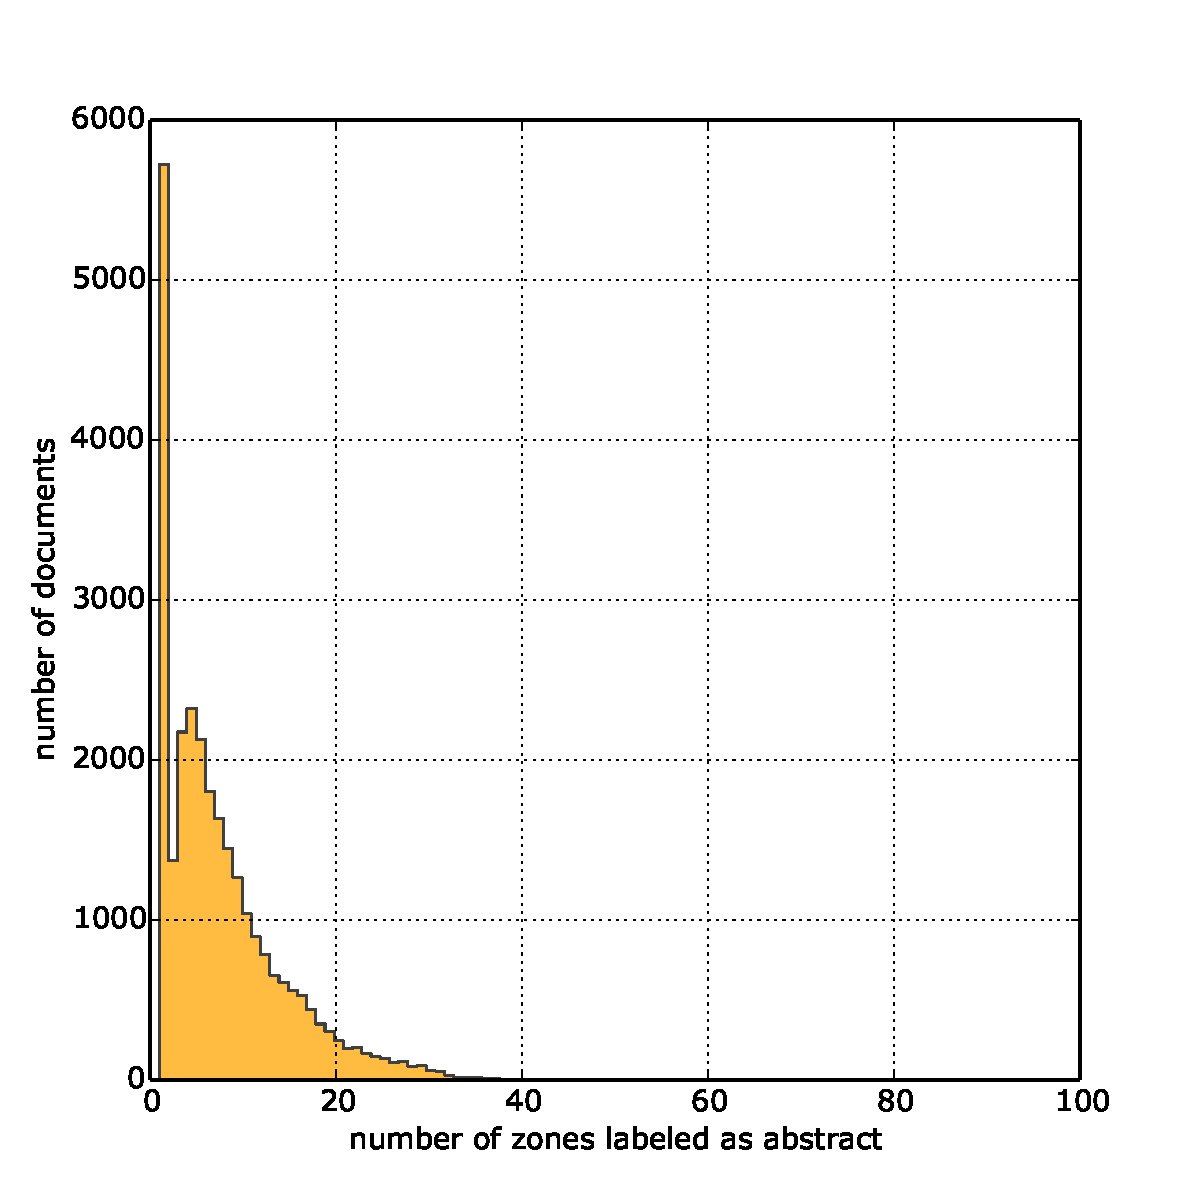
\includegraphics[width=8cm]{plots/abstract_histogram}
  \caption{Histogram of number of zones labeled as \texttt{abstract}}
  \label{fig:abstract_histogram}
\end{minipage}
\quad
\begin{minipage}[t!]{0.48\linewidth}
  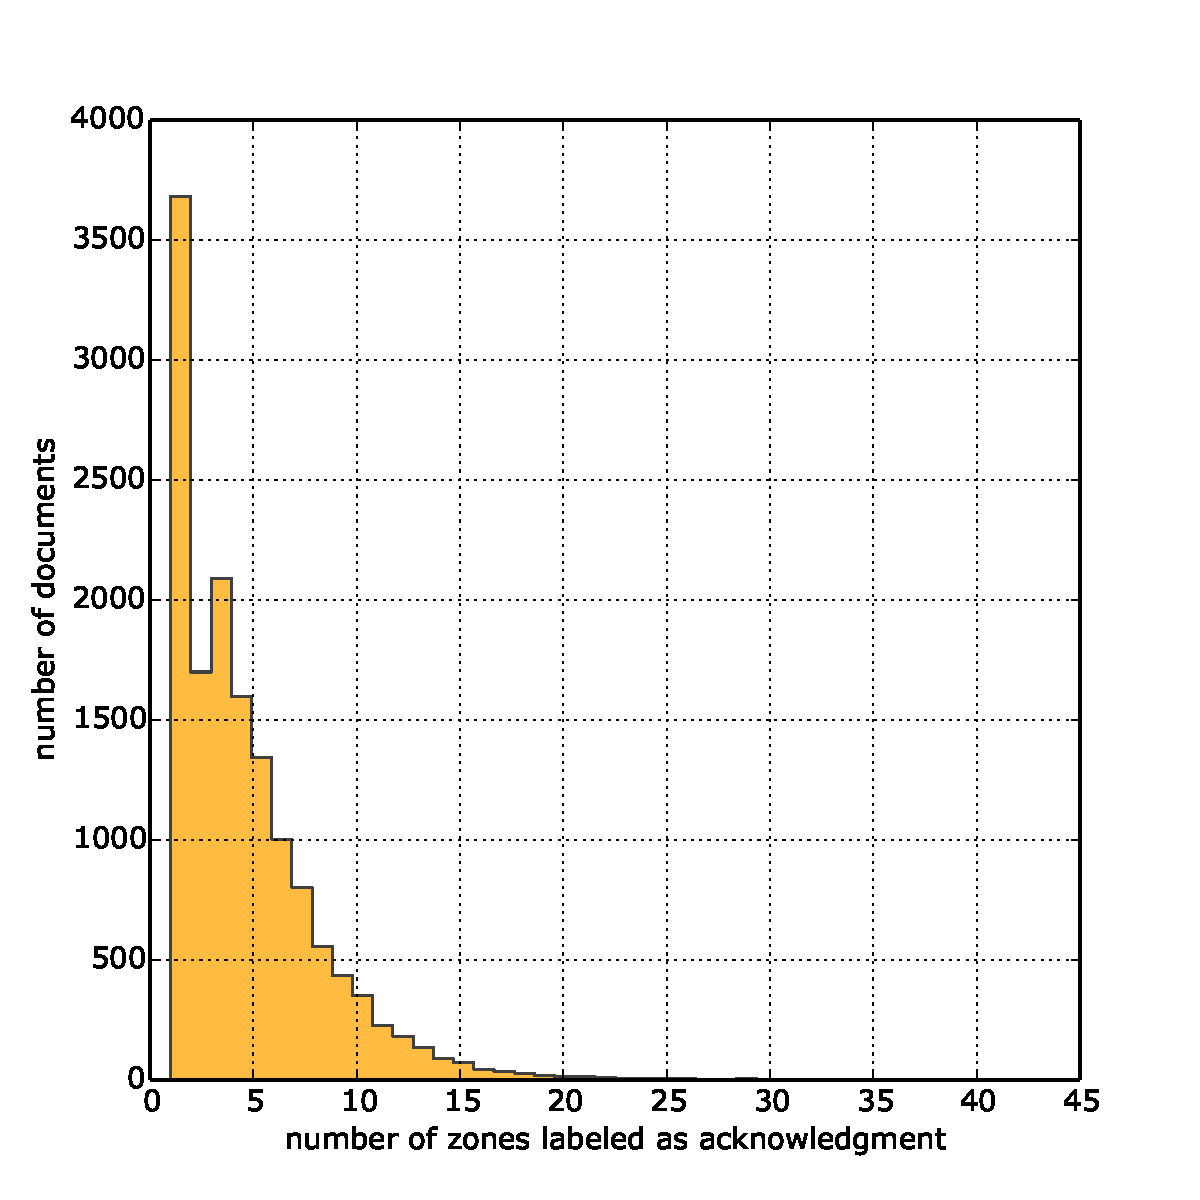
\includegraphics[width=8cm]{plots/acknowledgment_histogram}
  \caption{Histogram of number of zones labeled as \texttt{acknowledgment}}
  \label{fig:acknowledgment_histogram}
\end{minipage}
\end{figure}

\begin{figure}
\centering
\begin{minipage}[t!]{0.48\linewidth}
  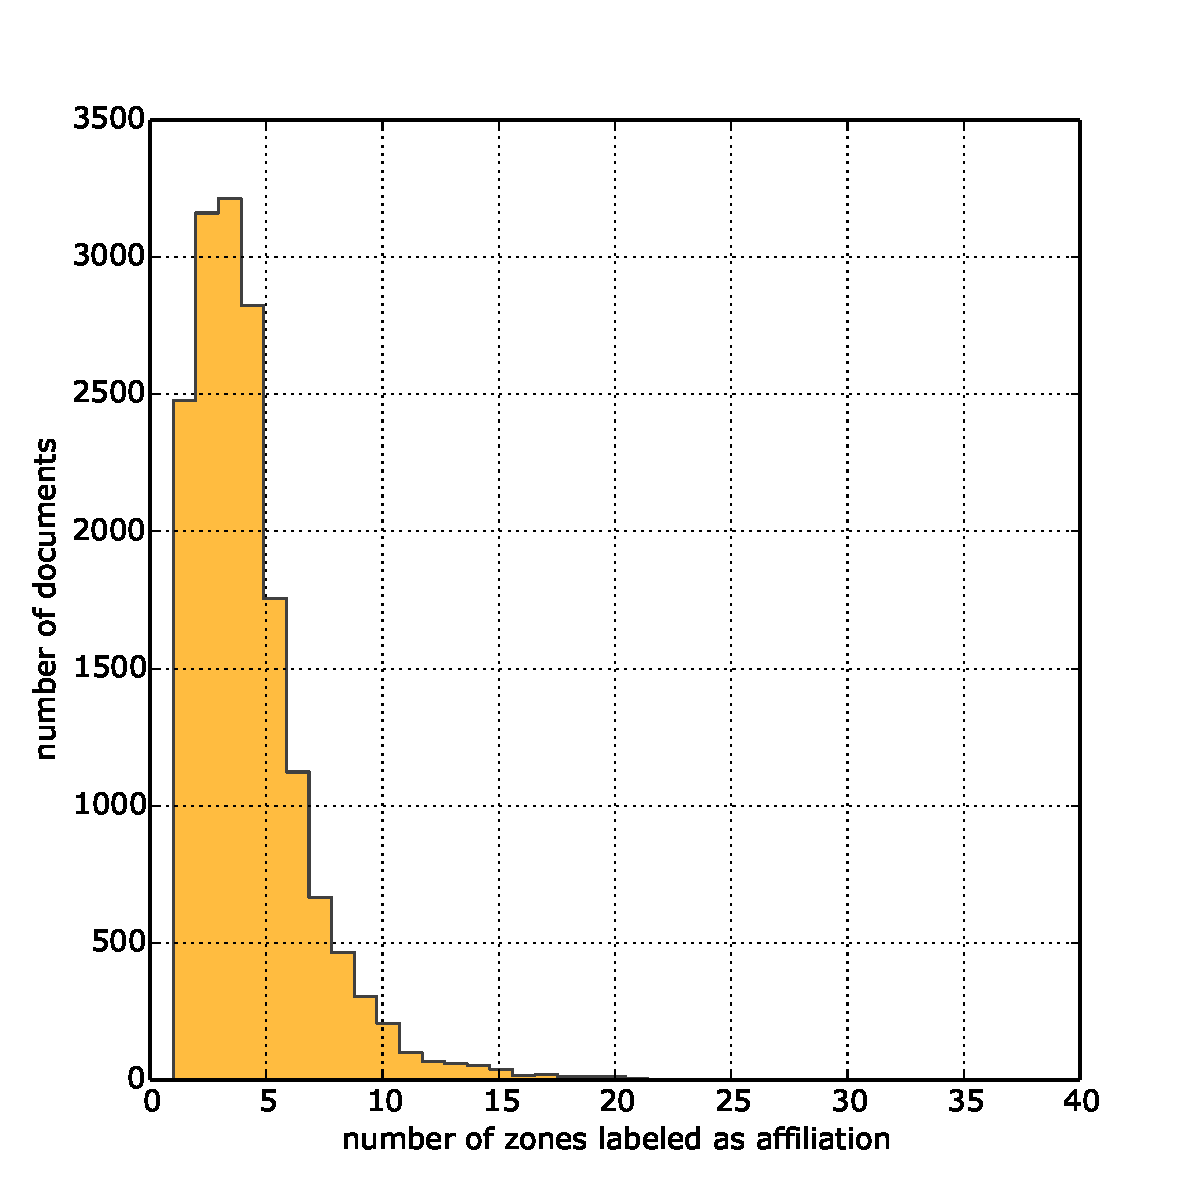
\includegraphics[width=8cm]{plots/affiliation_histogram}
  \caption{Histogram of number of zones labeled as \texttt{affiliation}}
  \label{fig:affiliation_histogram}
\end{minipage}
\quad
\begin{minipage}[t!]{0.48\linewidth}
  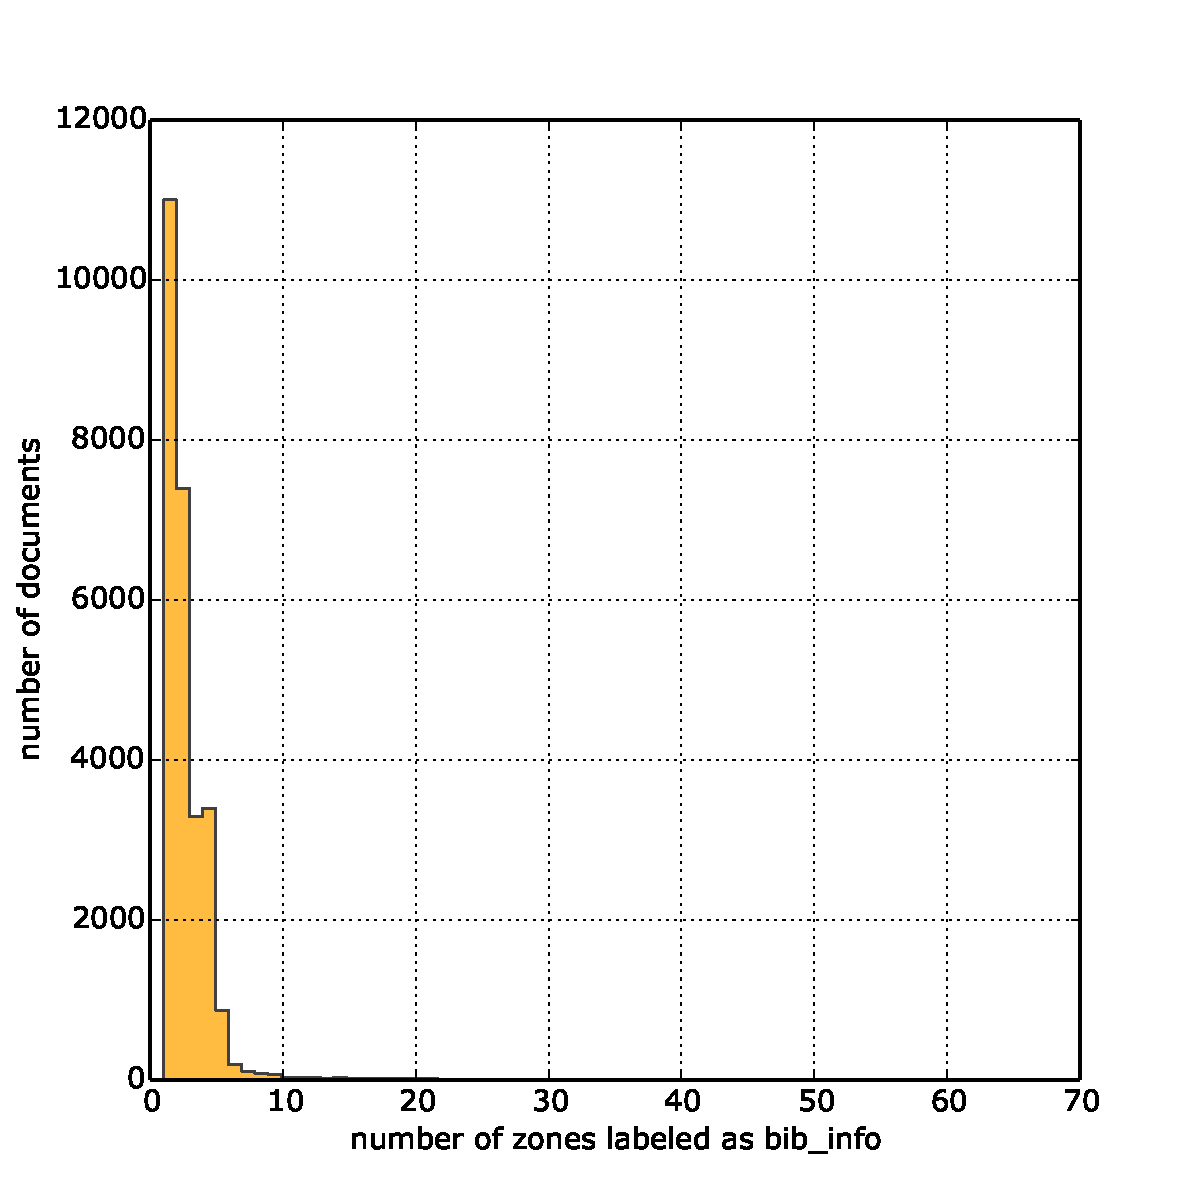
\includegraphics[width=8cm]{plots/bib_info_histogram}
  \caption{Histogram of number of zones labeled as \texttt{bib\_info}}
  \label{fig:bib_info_histogram}
\end{minipage}
\end{figure}

\begin{figure}
\centering
\begin{minipage}[t!]{0.48\linewidth}
  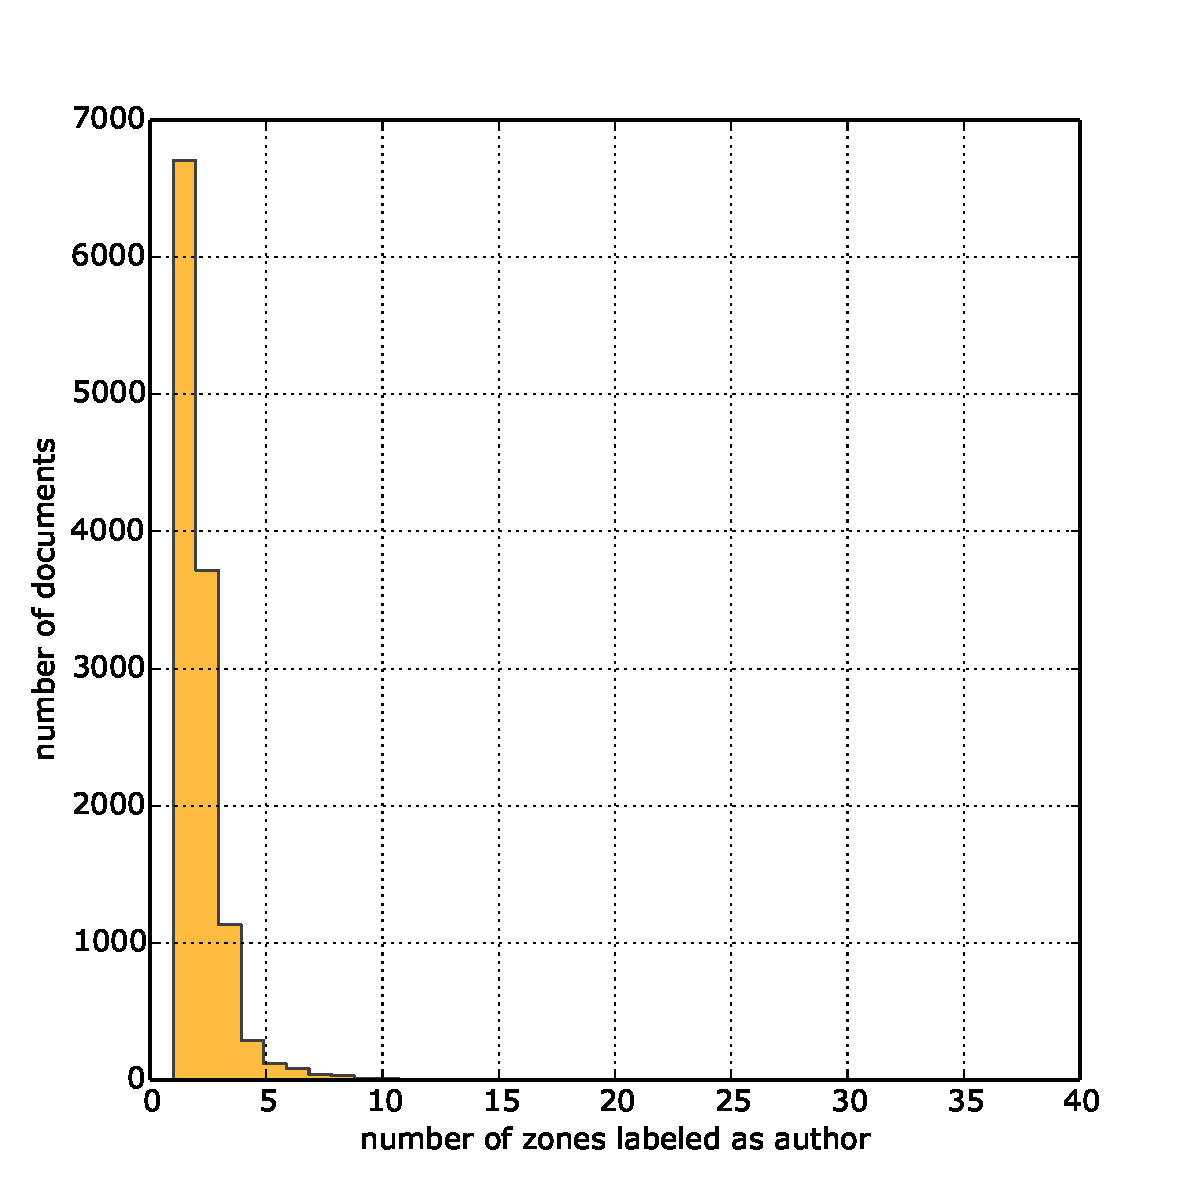
\includegraphics[width=8cm]{plots/author_histogram}
  \caption{Histogram of number of zones labeled as \texttt{author}}
  \label{fig:author_histogram}
\end{minipage}
\quad
\begin{minipage}[t!]{0.48\linewidth}
  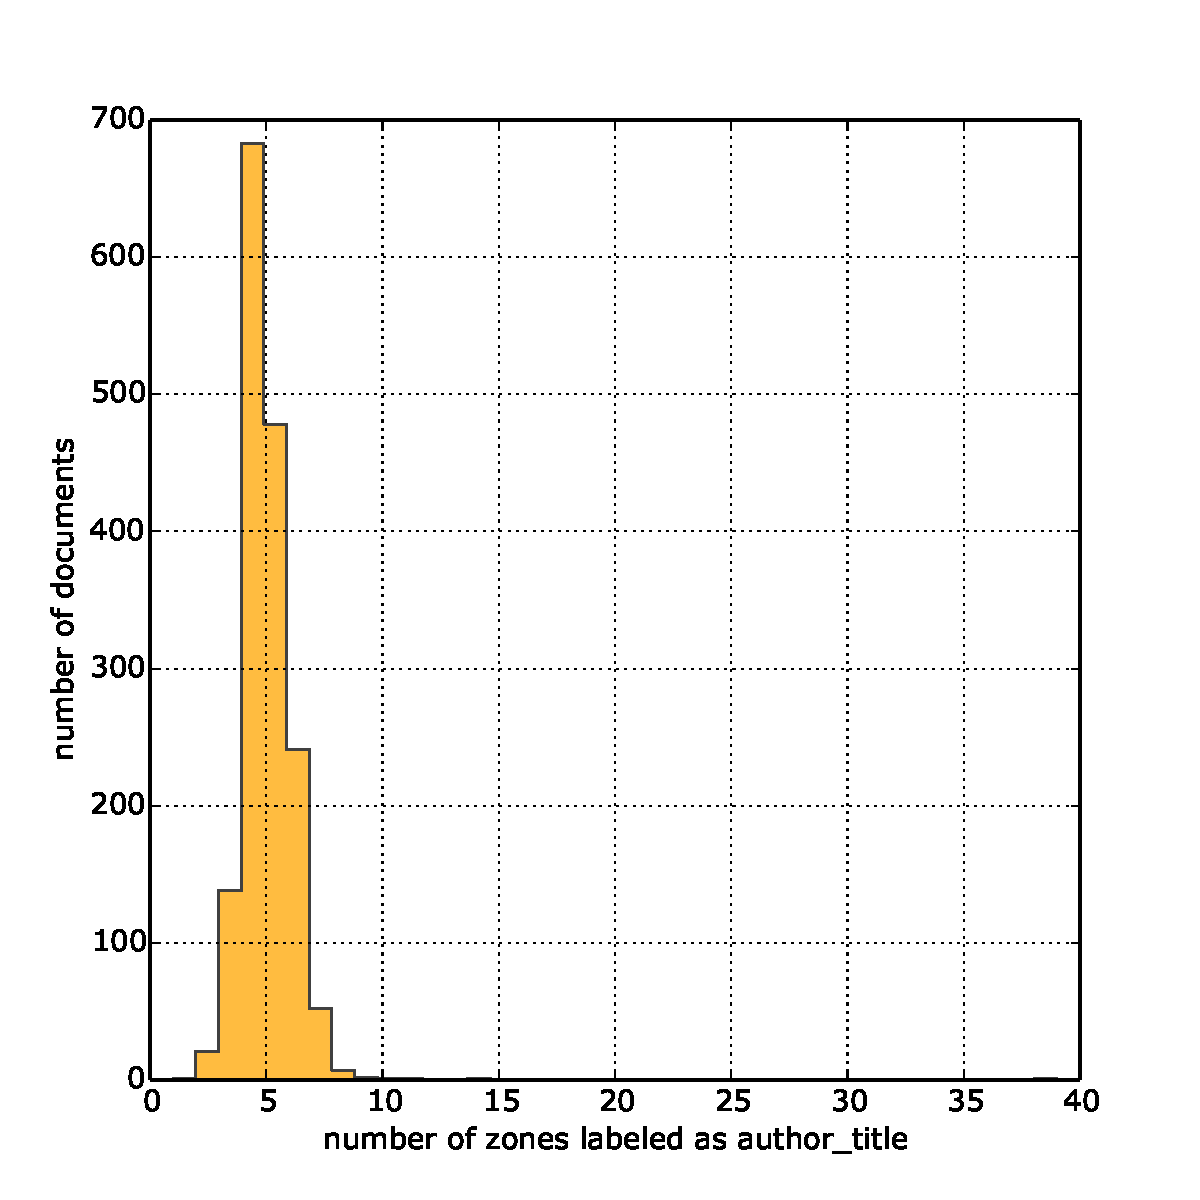
\includegraphics[width=8cm]{plots/author_title_histogram}
  \caption{Histogram of number of zones labeled as \texttt{author\_title}}
  \label{fig:author_title_histogram}
\end{minipage}
\end{figure}

\begin{figure}
\centering
\begin{minipage}[t!]{0.48\linewidth}
  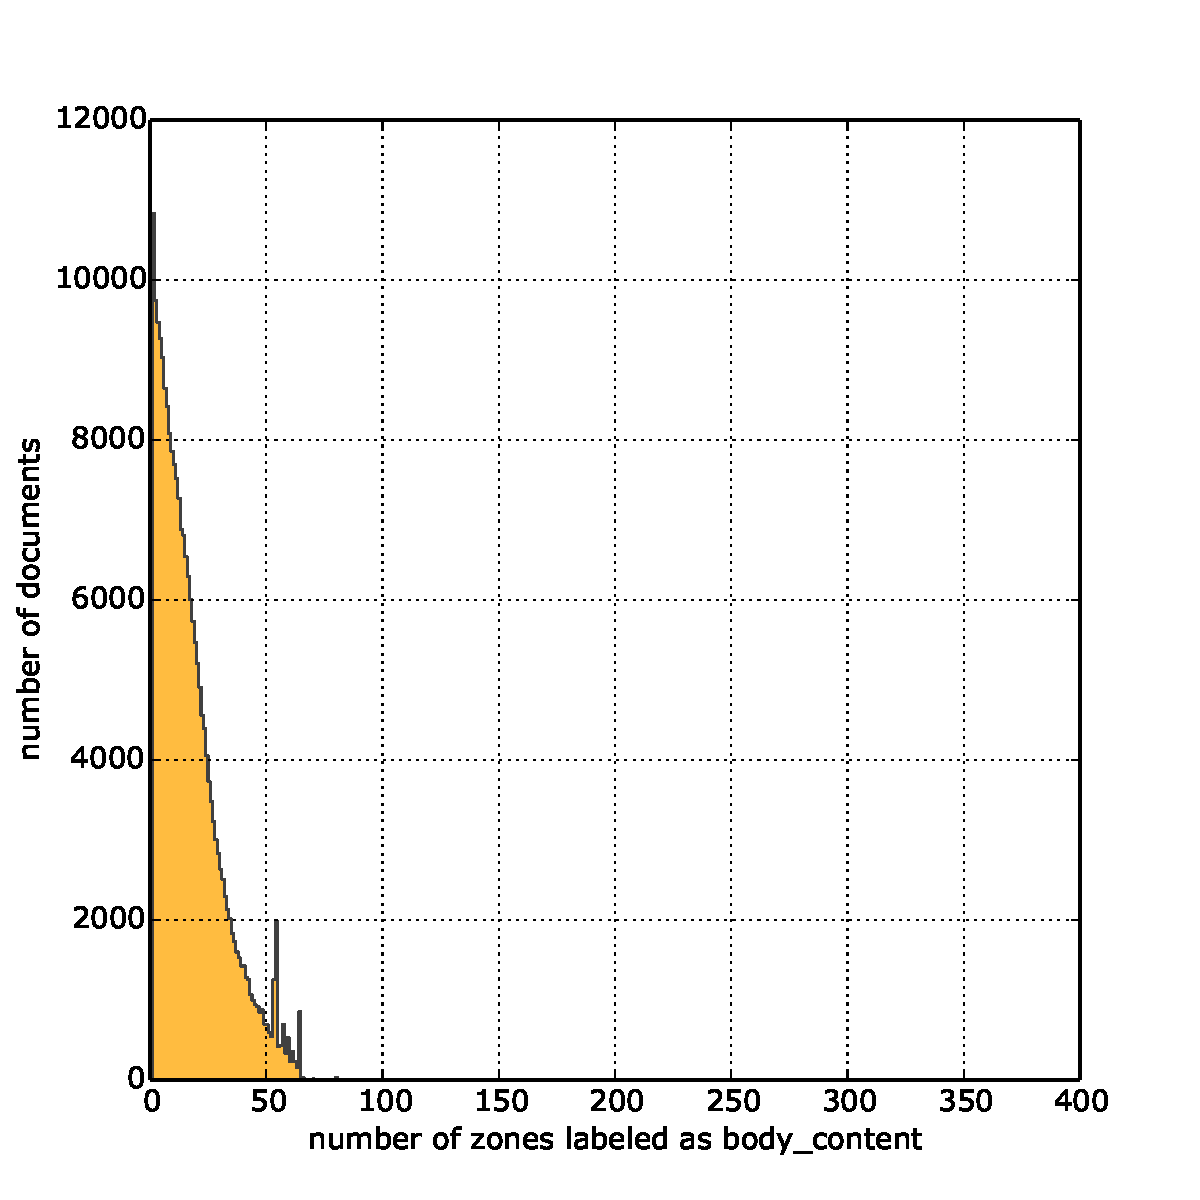
\includegraphics[width=8cm]{plots/body_content_histogram}
  \caption{Histogram of number of zones labeled as \texttt{body\_content}}
  \label{fig:body_content_histogram}
\end{minipage}
\quad
\begin{minipage}[t!]{0.48\linewidth}
  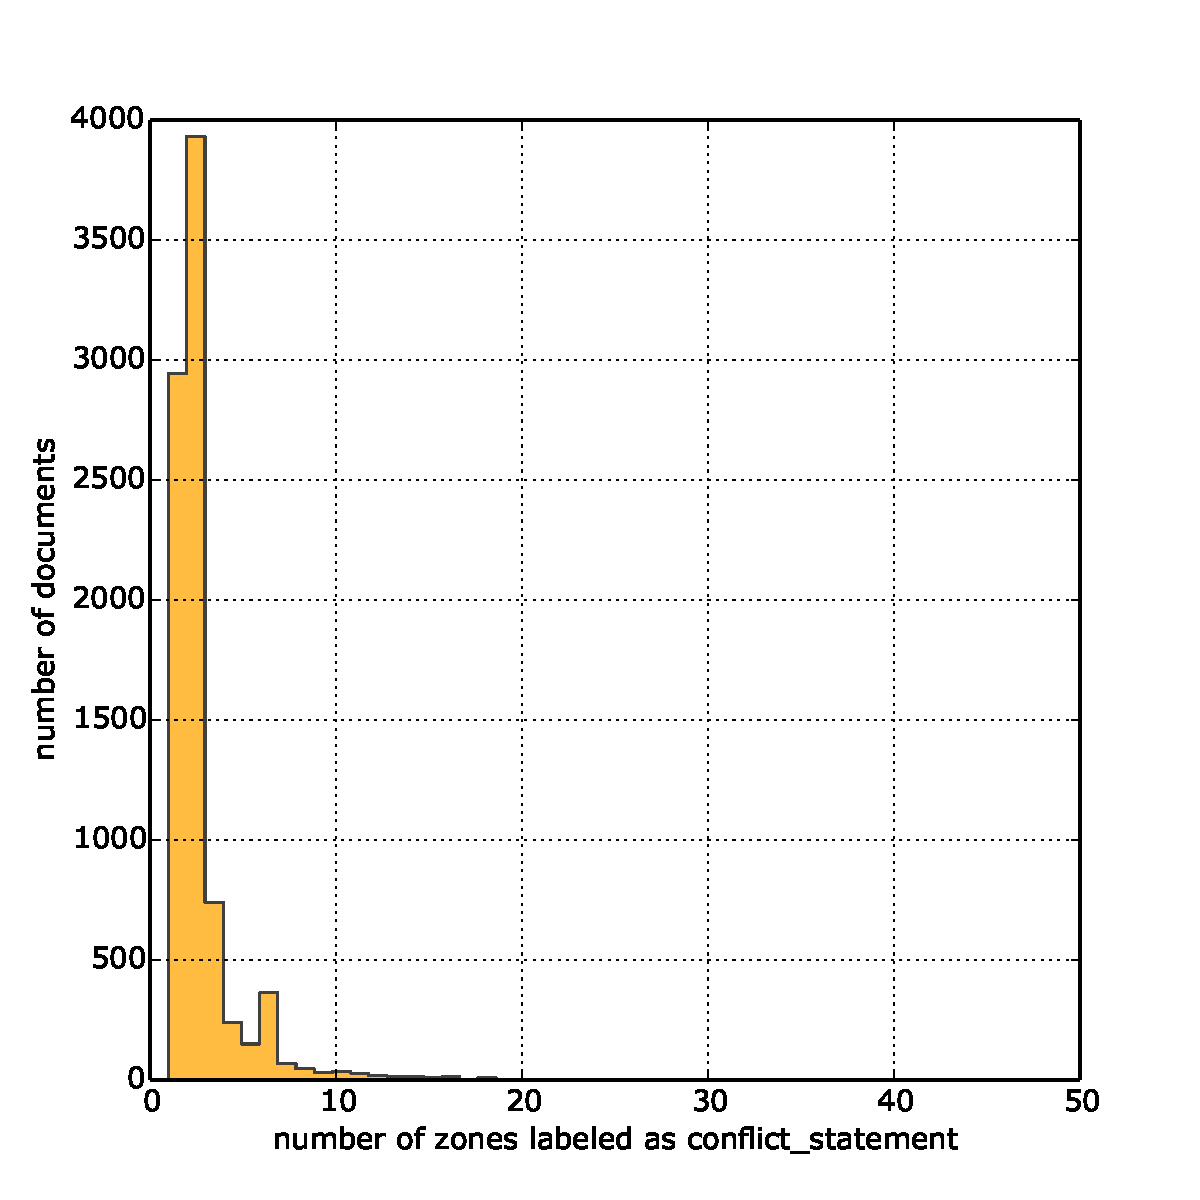
\includegraphics[width=8cm]{plots/conflict_statement_histogram}
  \caption{Histogram of number of zones labeled as \texttt{conflict\_statement}}
  \label{fig:conflict_statement_histogram}
\end{minipage}
\end{figure}

\begin{figure}
\centering
\begin{minipage}[t!]{0.48\linewidth}
  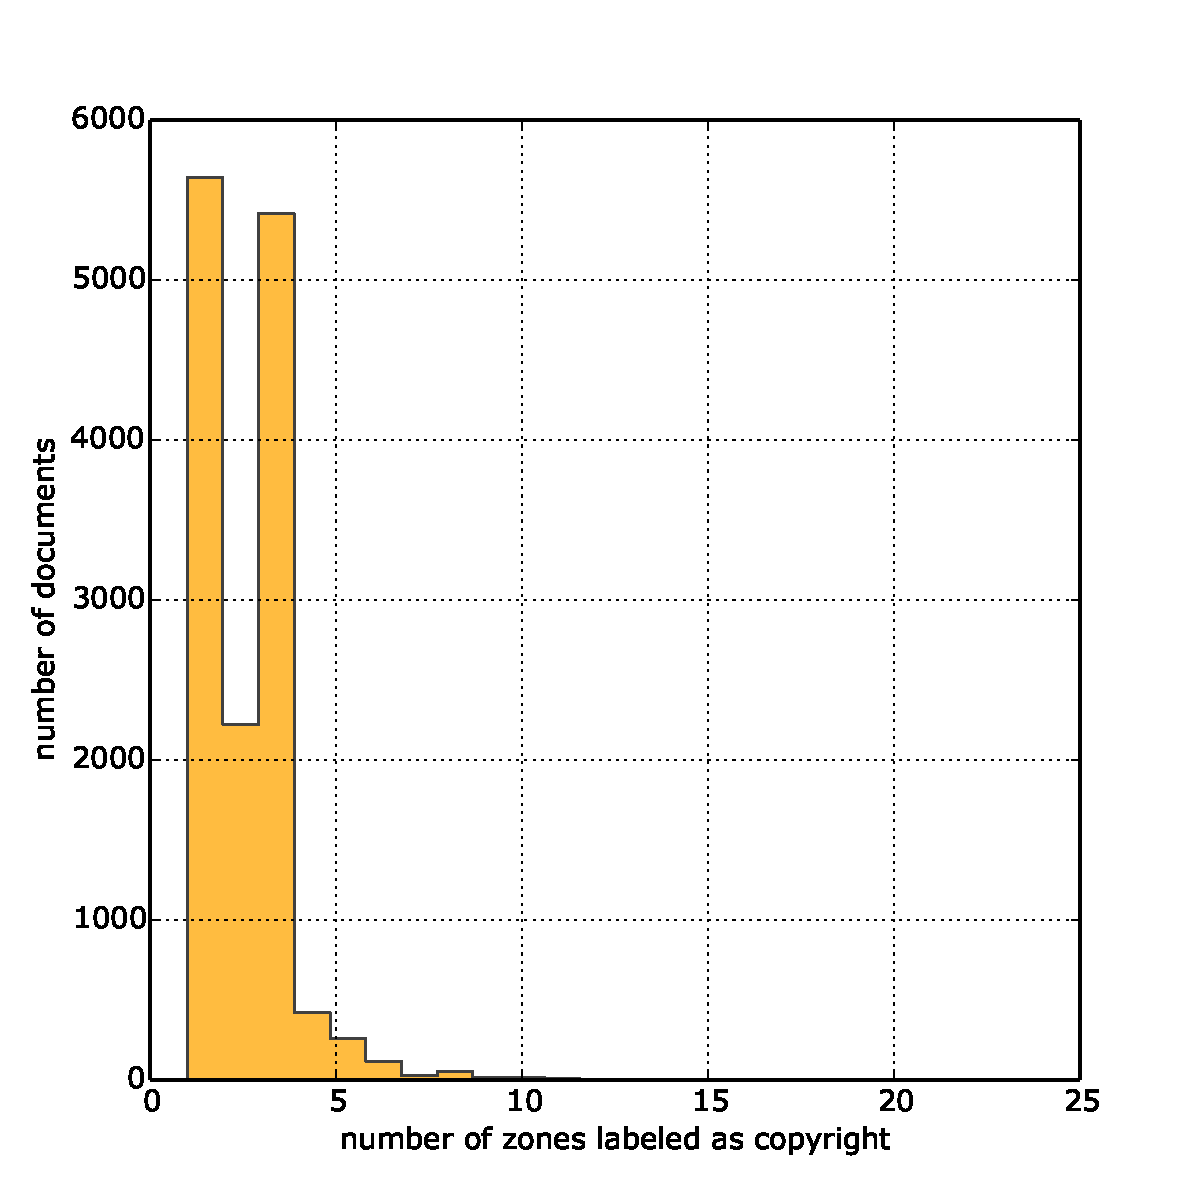
\includegraphics[width=8cm]{plots/copyright_histogram}
  \caption{Histogram of number of zones labeled as \texttt{copyright}}
  \label{fig:copyright_histogram}
\end{minipage}
\quad
\begin{minipage}[t!]{0.48\linewidth}
  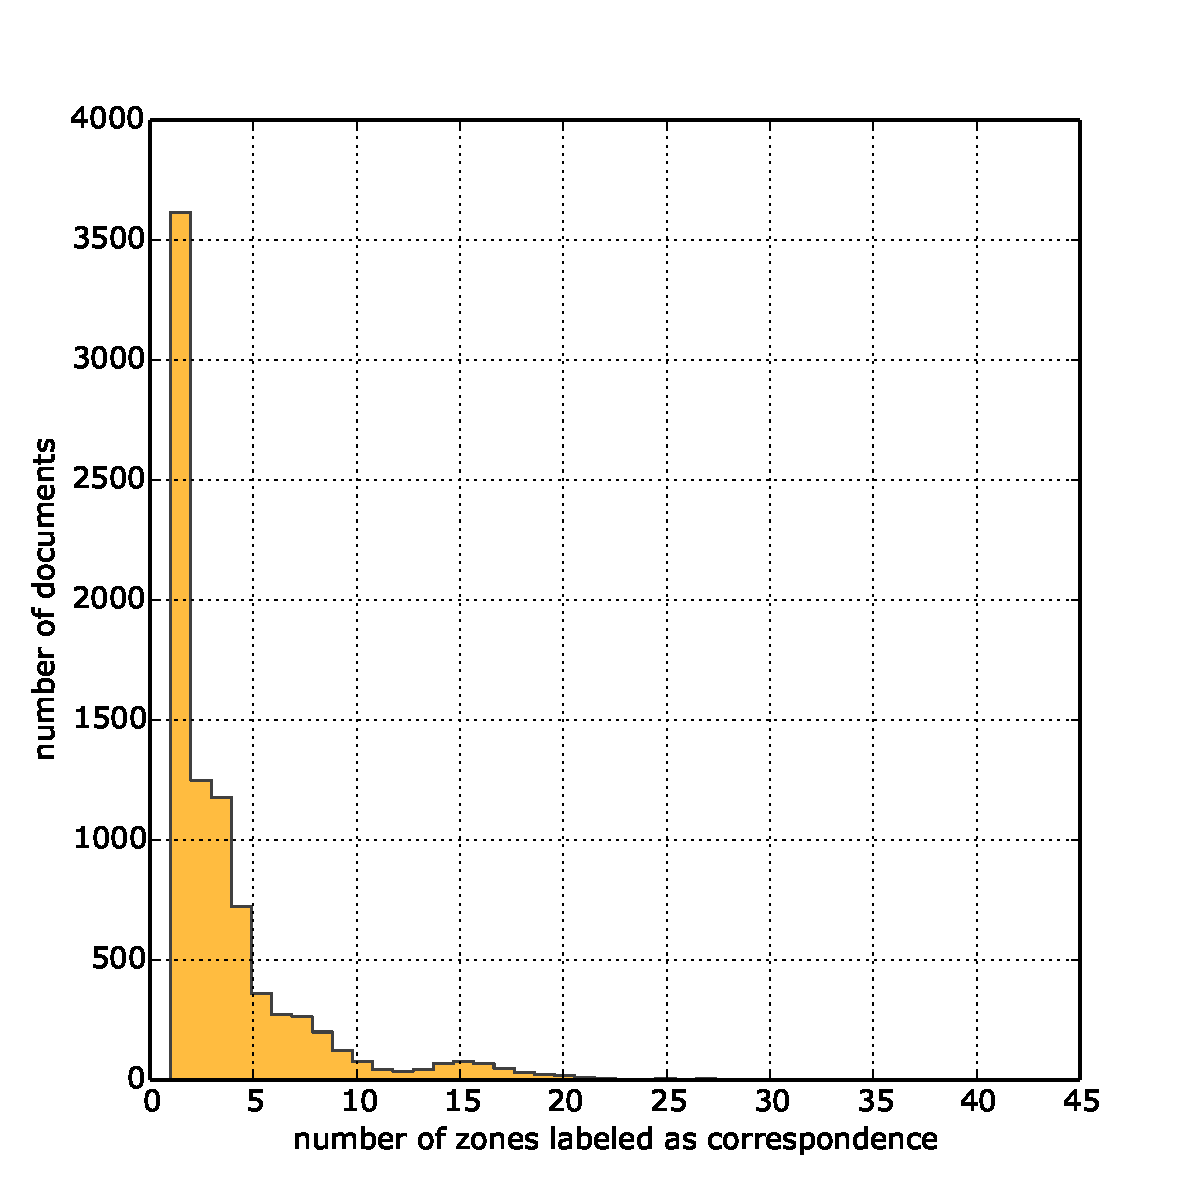
\includegraphics[width=8cm]{plots/correspondence_histogram}
  \caption{Histogram of number of zones labeled as \texttt{correspondence}}
  \label{fig:correspondence_histogram}
\end{minipage}
\end{figure}

\begin{figure}
\centering
\begin{minipage}[t!]{0.48\linewidth}
  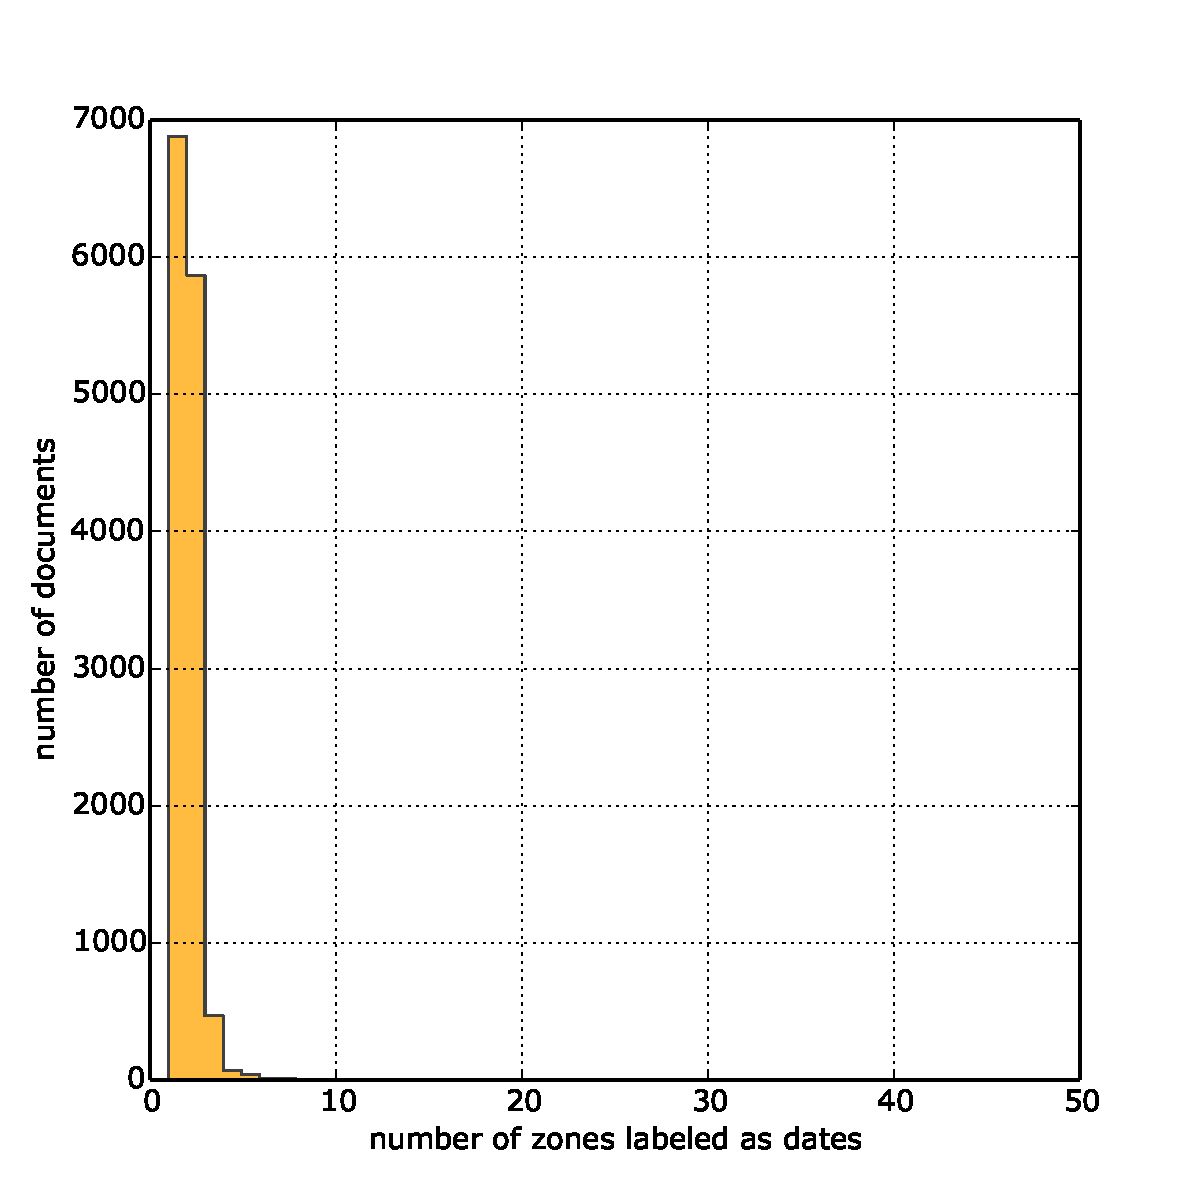
\includegraphics[width=8cm]{plots/dates_histogram}
  \caption{Histogram of number of zones labeled as \texttt{dates}}
  \label{fig:dates_histogram}
\end{minipage}
\quad
\begin{minipage}[t!]{0.48\linewidth}
  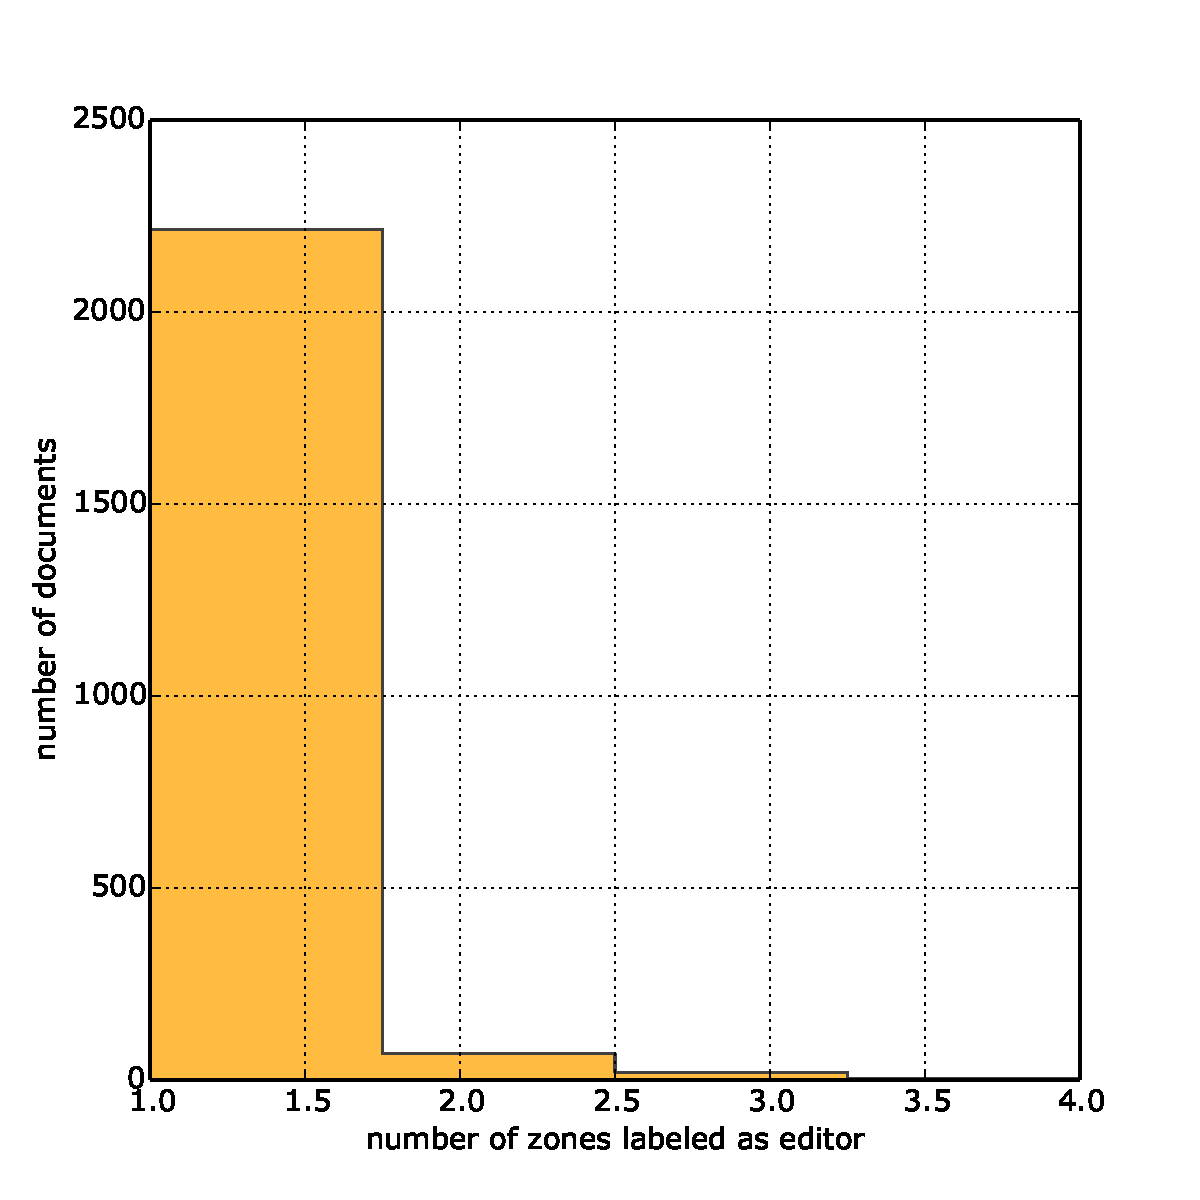
\includegraphics[width=8cm]{plots/editor_histogram}
  \caption{Histogram of number of zones labeled as \texttt{editor}}
  \label{fig:editor_histogram}
\end{minipage}
\end{figure}

  \begin{figure}
\centering
\begin{minipage}[t!]{0.48\linewidth}
  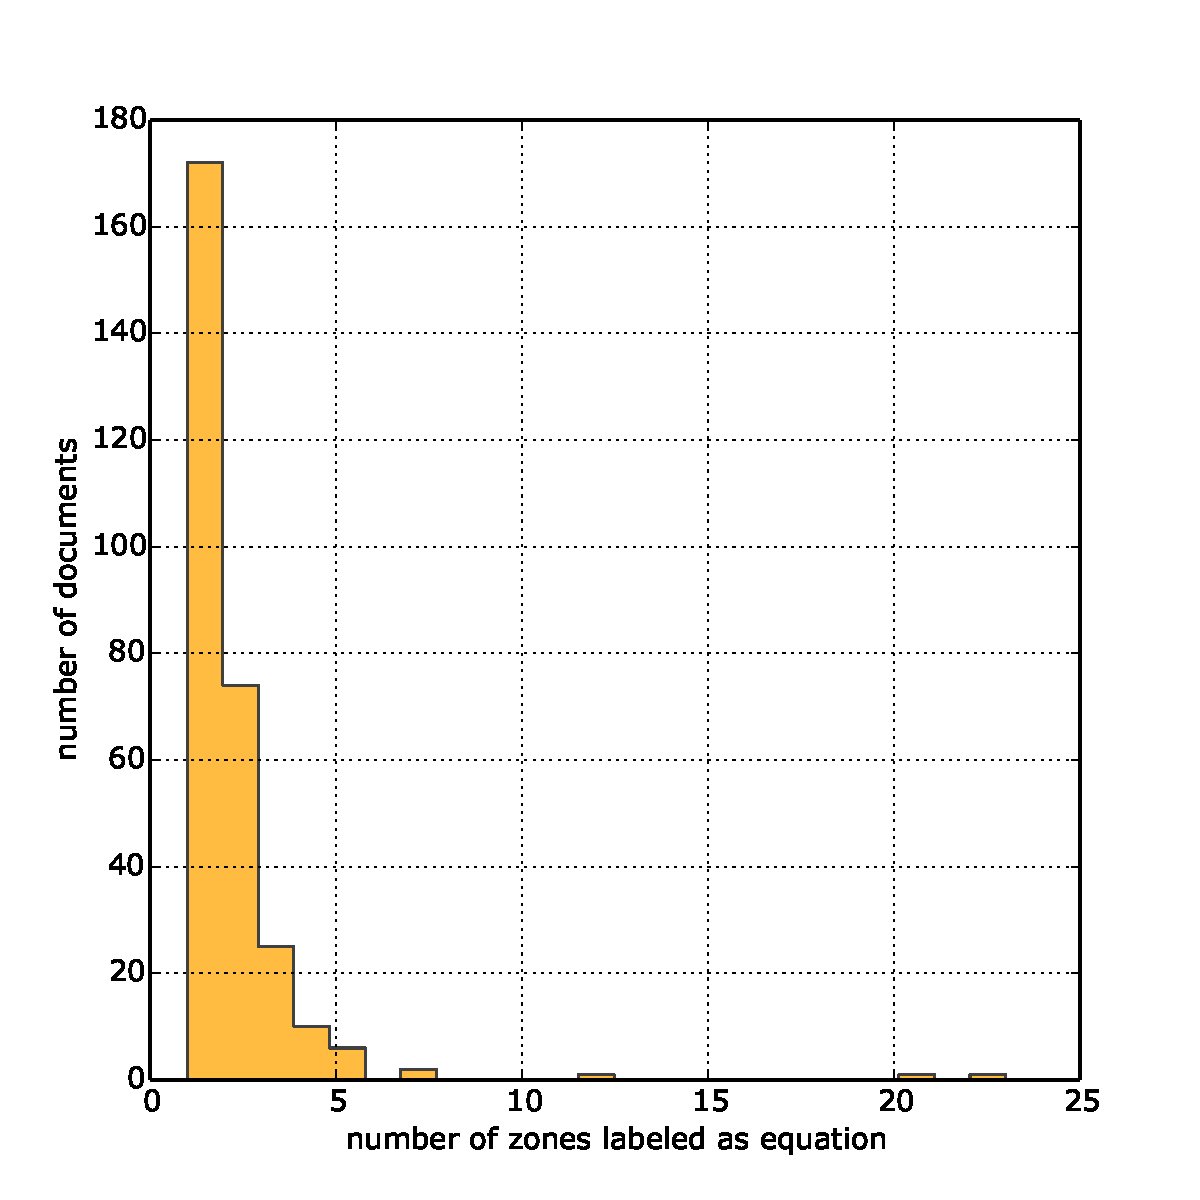
\includegraphics[width=8cm]{plots/equation_histogram}
  \caption{Histogram of number of zones labeled as \texttt{equation}}
  \label{fig:equation_histogram}
\end{minipage}
\quad
\begin{minipage}[t!]{0.48\linewidth}
  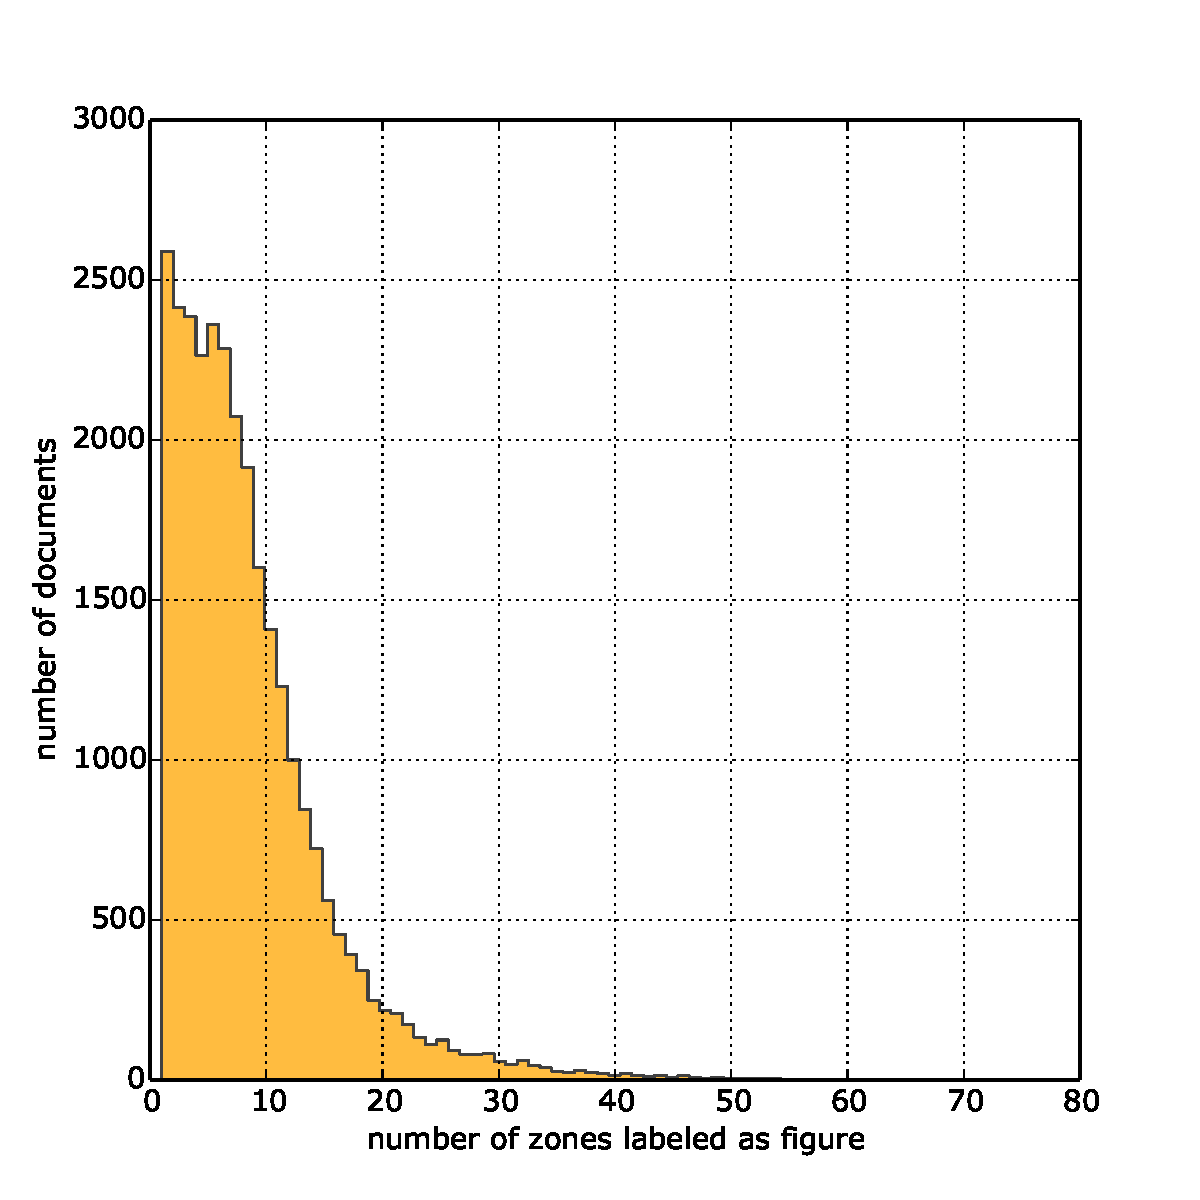
\includegraphics[width=8cm]{plots/figure_histogram}
  \caption{Histogram of number of zones labeled as \texttt{figure}}
  \label{fig:figure_histogram}
\end{minipage}
\end{figure}

\begin{figure}
\centering
\begin{minipage}[t!]{0.48\linewidth}
  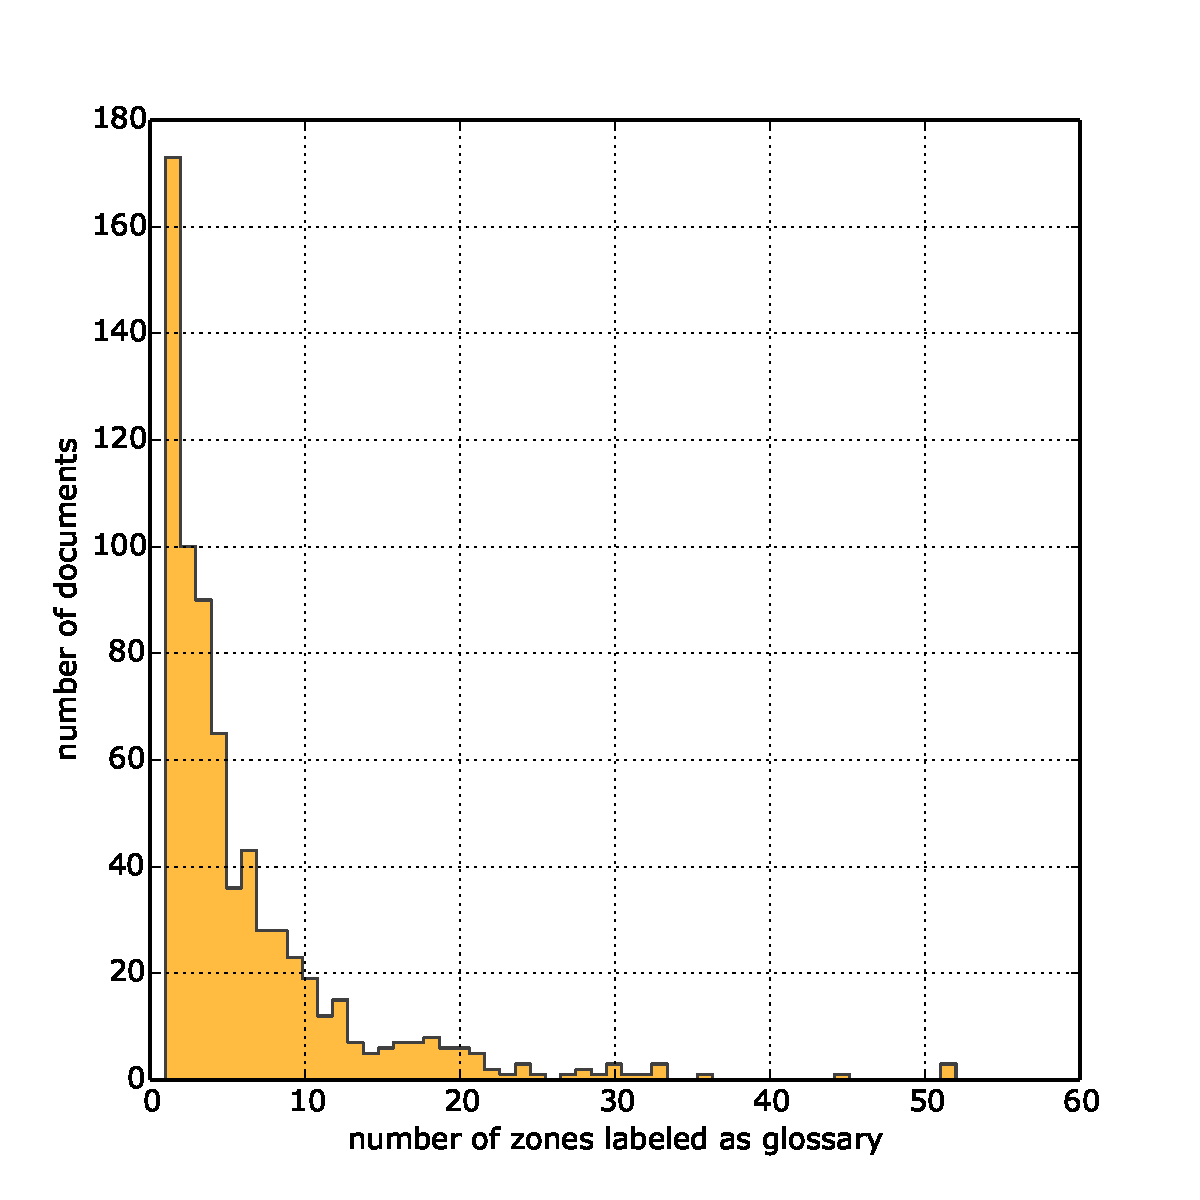
\includegraphics[width=8cm]{plots/glossary_histogram}
  \caption{Histogram of number of zones labeled as \texttt{glossary}}
  \label{fig:glossary_histogram}
\end{minipage}
\quad
\begin{minipage}[t!]{0.48\linewidth}
  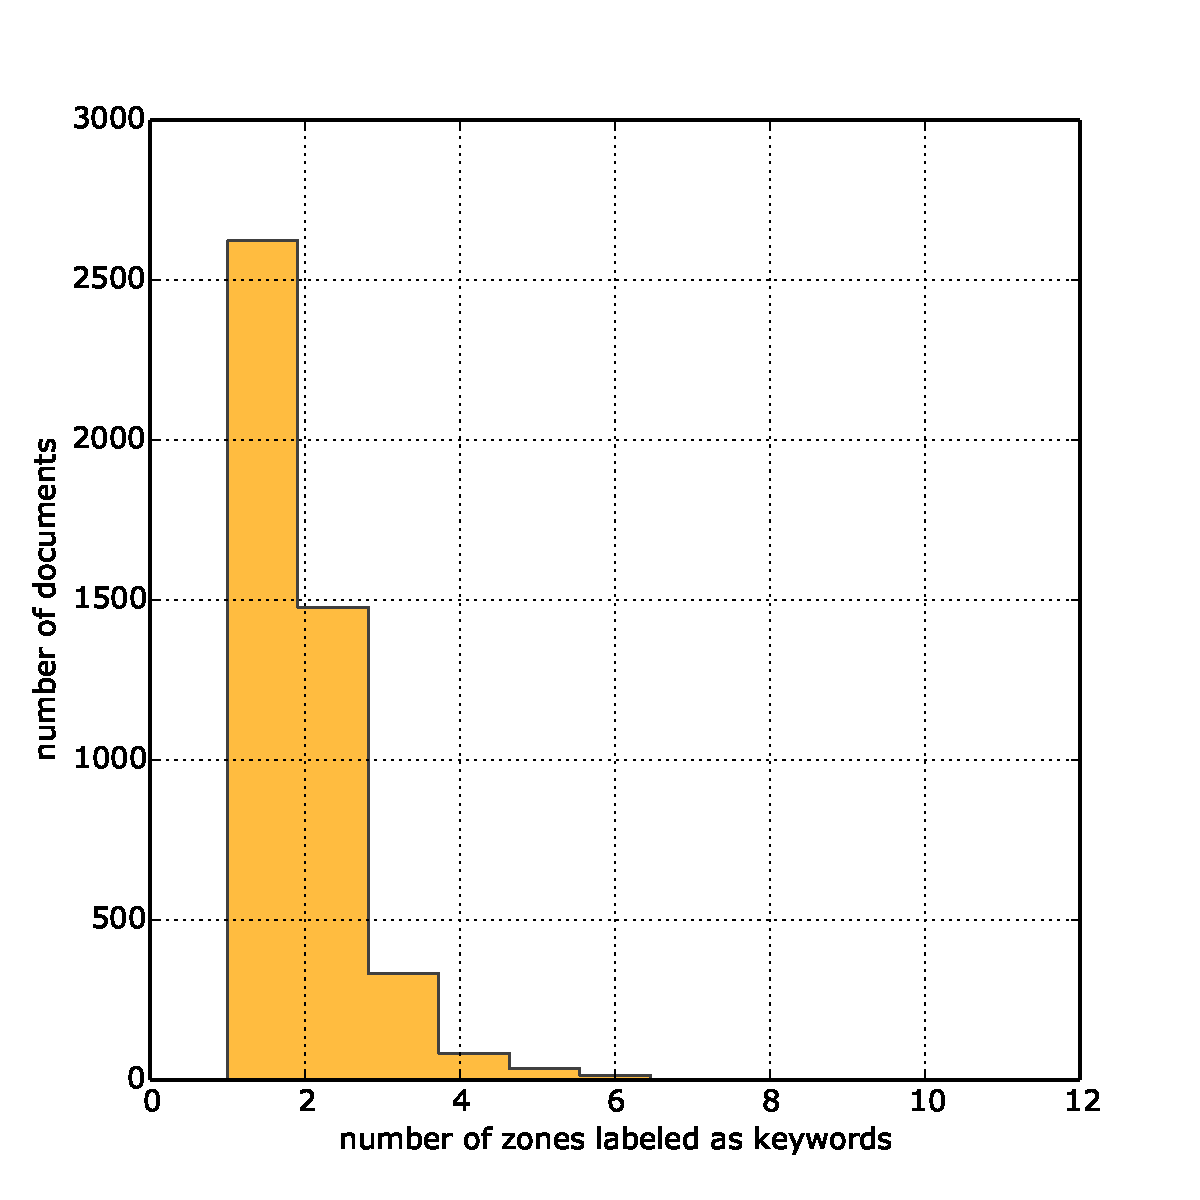
\includegraphics[width=8cm]{plots/keywords_histogram}
  \caption{Histogram of number of zones labeled as \texttt{keywords}}
  \label{fig:keywords_histogram}
\end{minipage}
\end{figure}

\begin{figure}
\centering
\begin{minipage}[t!]{0.48\linewidth}
  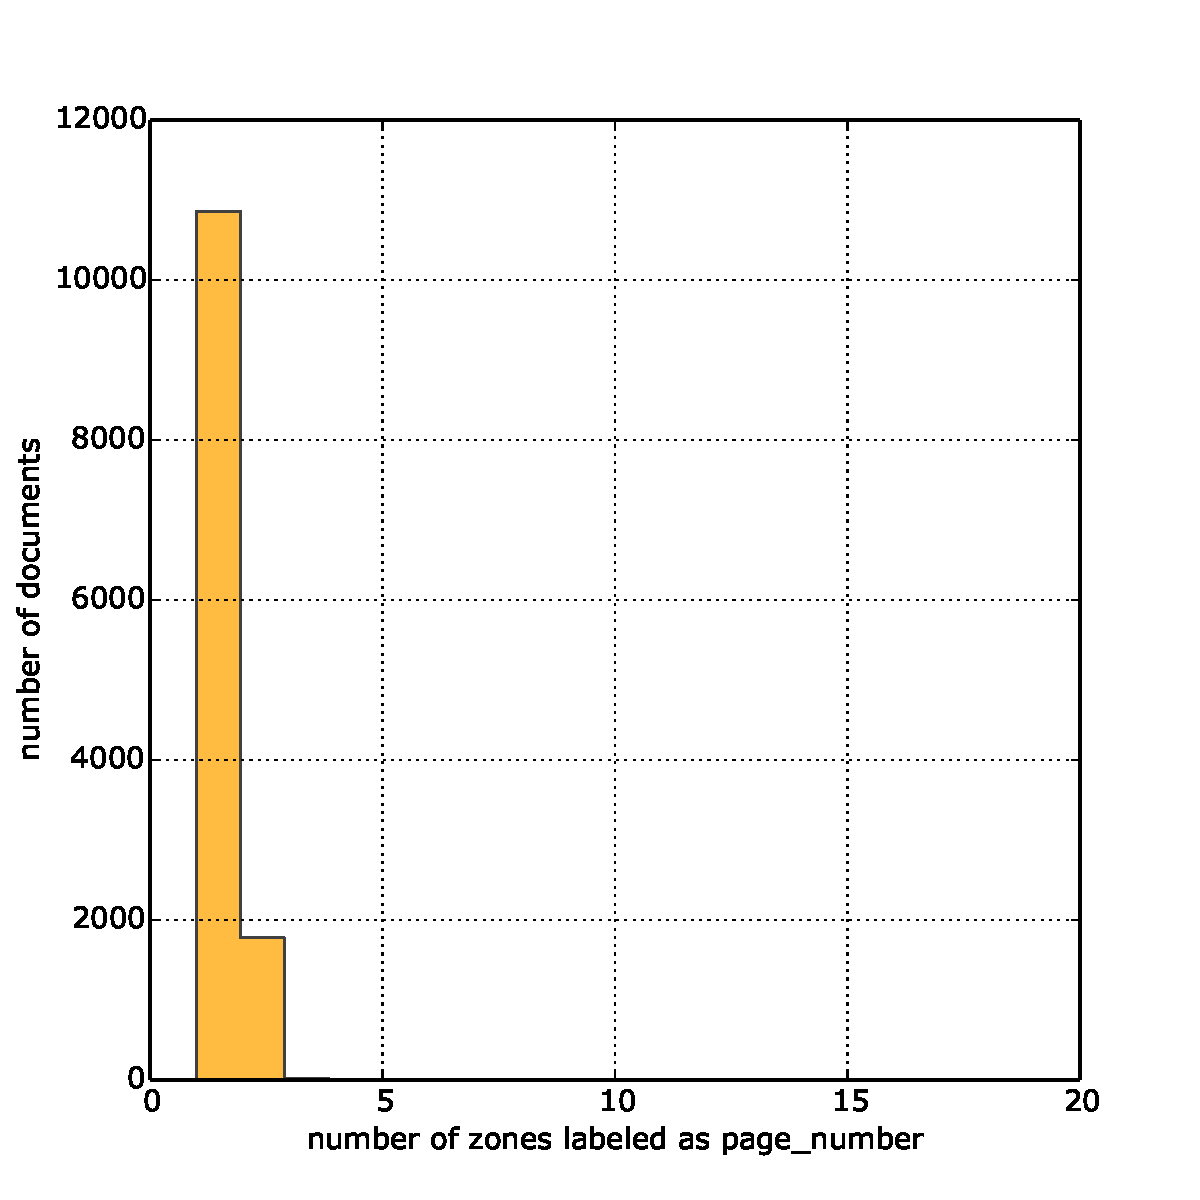
\includegraphics[width=8cm]{plots/page_number_histogram}
  \caption{Histogram of number of zones labeled as \texttt{page\_number}}
  \label{fig:page_number_histogram}
\end{minipage}
\quad
\begin{minipage}[t!]{0.48\linewidth}
  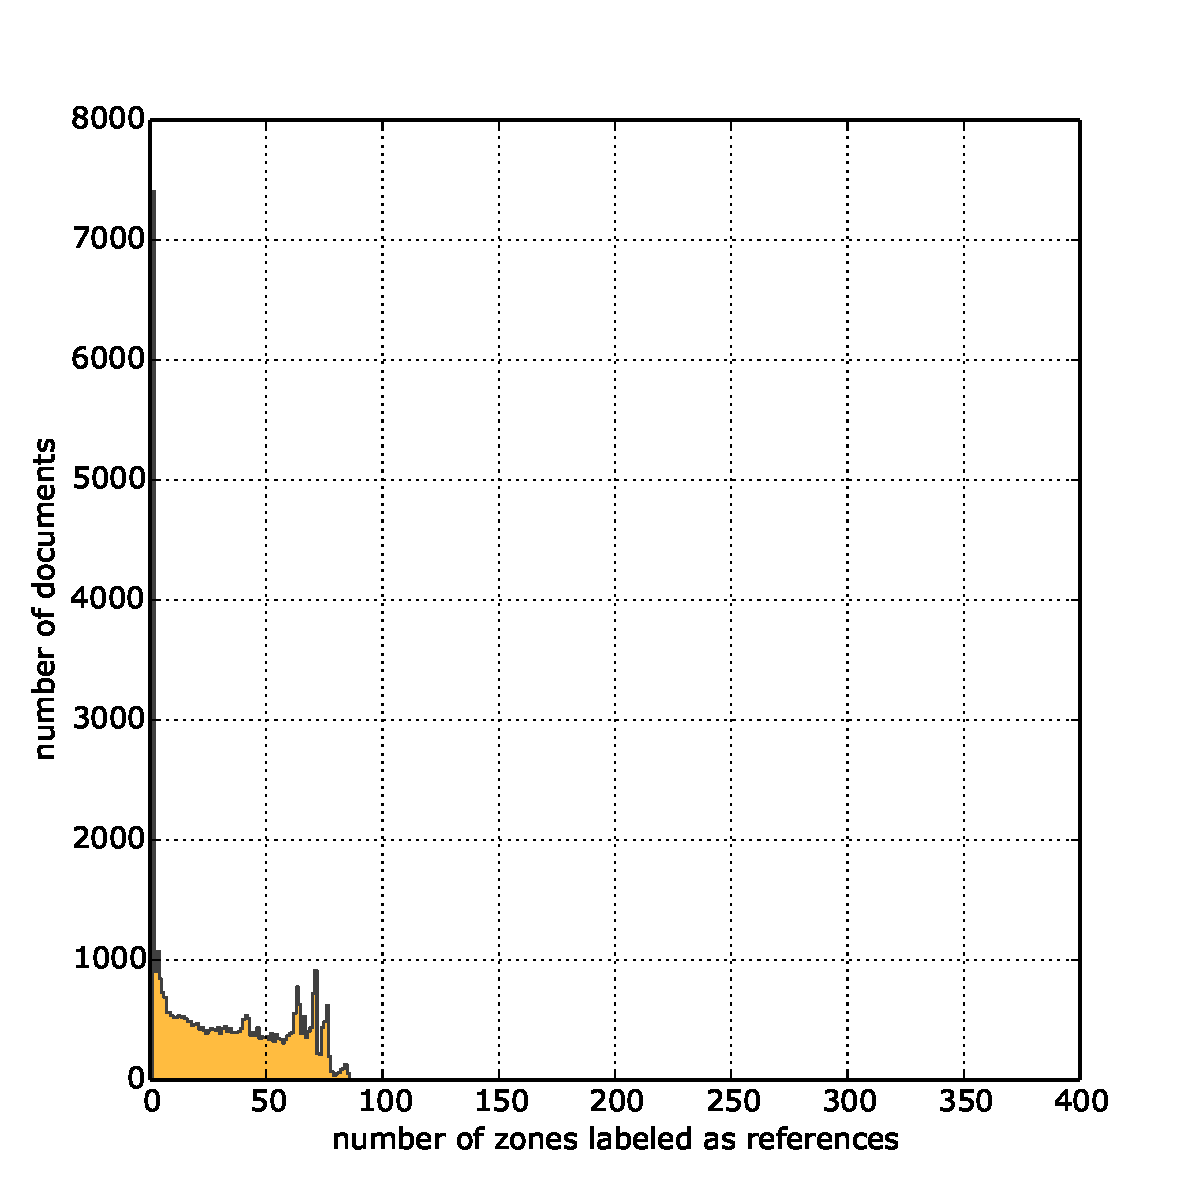
\includegraphics[width=8cm]{plots/references_histogram}
  \caption{Histogram of number of zones labeled as \texttt{reference}}
  \label{fig:reference_histogram}
\end{minipage}
\end{figure}

  \begin{figure}
\centering
\begin{minipage}[t!]{0.48\linewidth}
  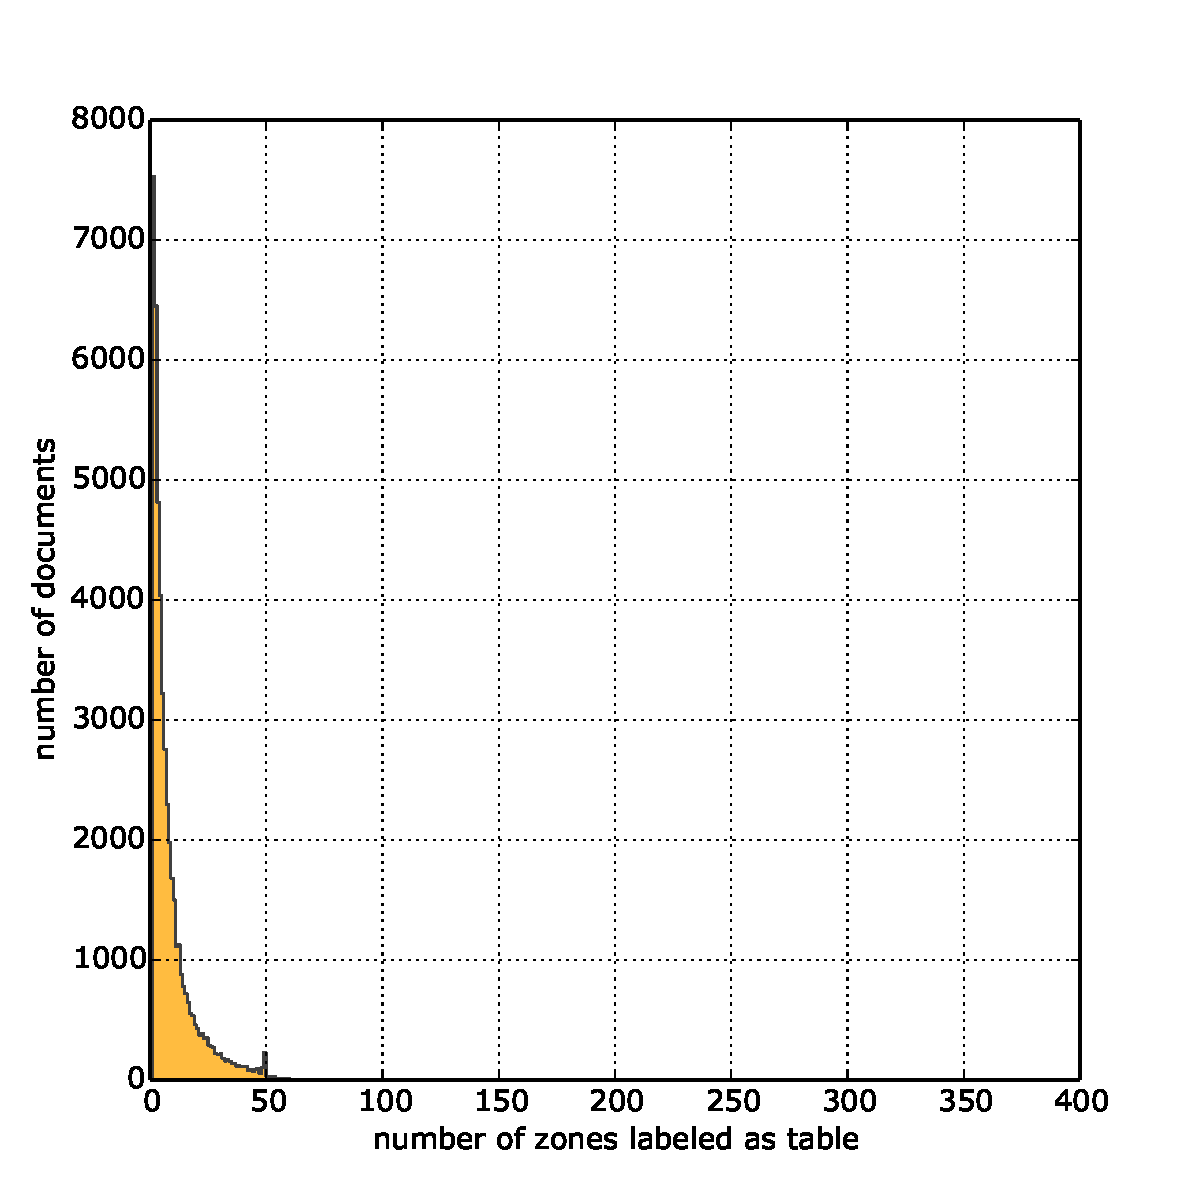
\includegraphics[width=8cm]{plots/table_histogram}
  \caption{Histogram of number of zones labeled as \texttt{table}}
  \label{fig:table_histogram}
\end{minipage}
\quad
\begin{minipage}[t!]{0.48\linewidth}
  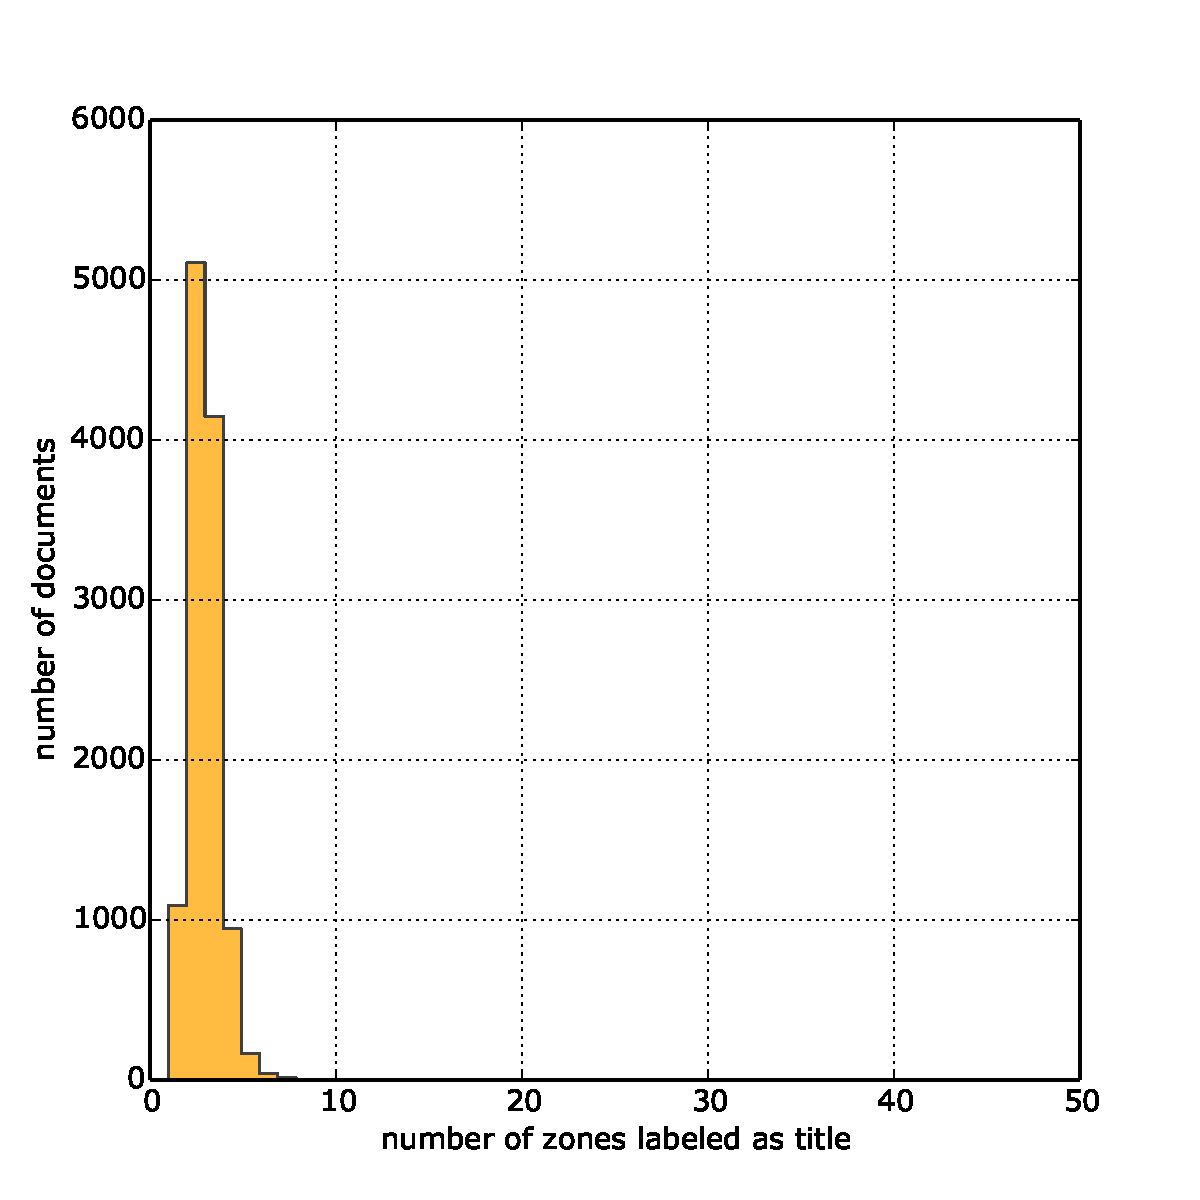
\includegraphics[width=8cm]{plots/title_histogram}
  \caption{Histogram of number of zones labeled as \texttt{title}}
  \label{fig:title_histogram}
\end{minipage}
\end{figure}

  \begin{figure}
\centering
\begin{minipage}[t!]{0.48\linewidth}
  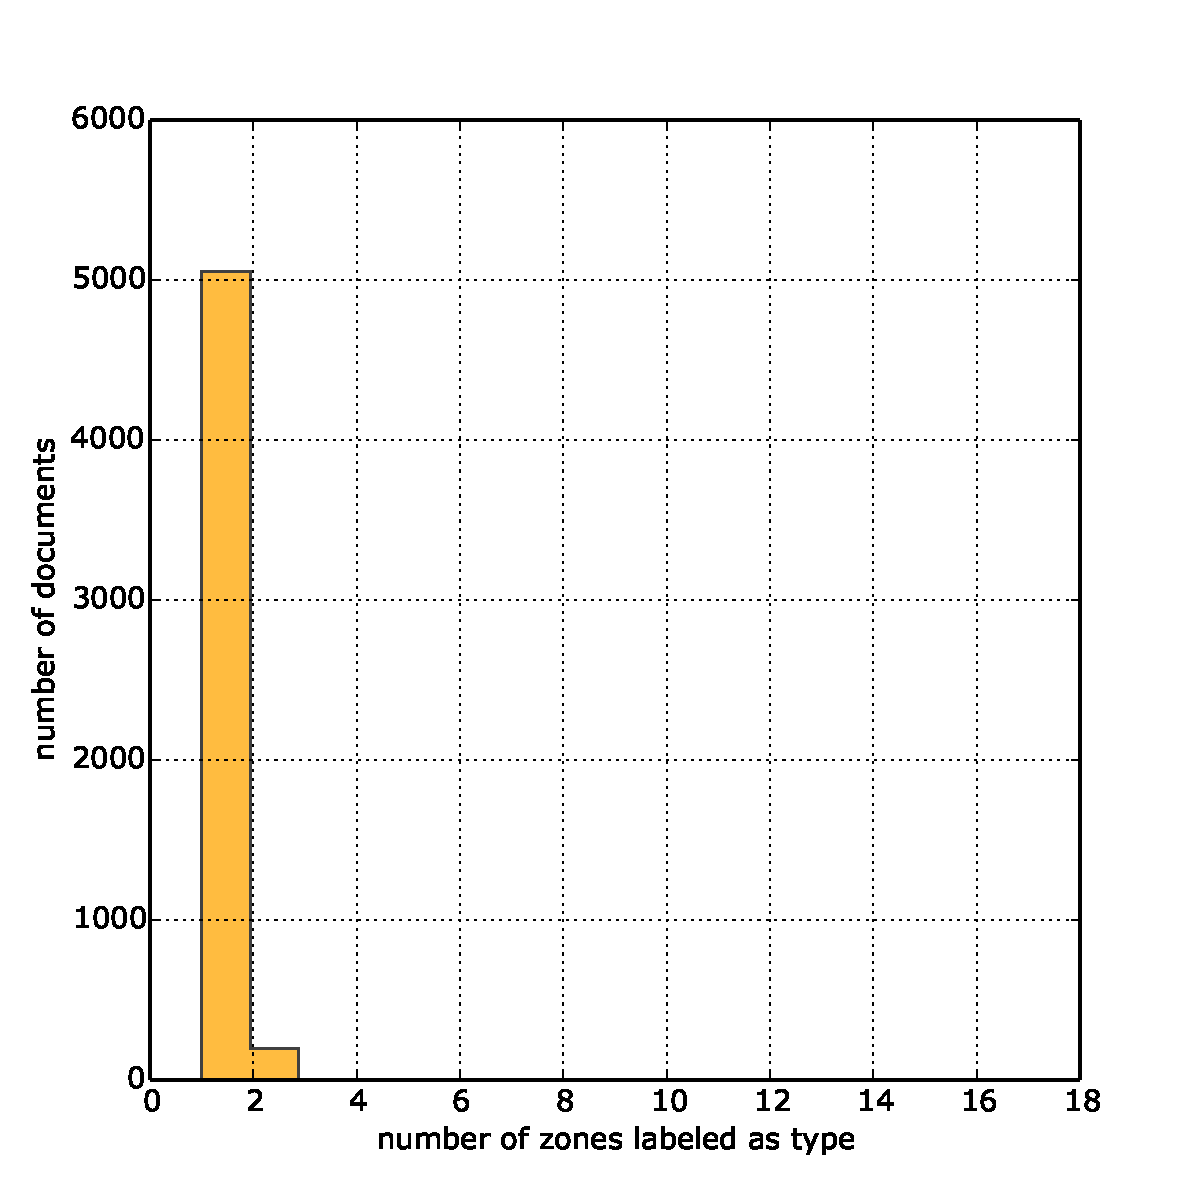
\includegraphics[width=8cm]{plots/type_histogram}
  \caption{Histogram of number of zones labeled as \texttt{type}}
  \label{fig:type_histogram}
\end{minipage}
\quad
\begin{minipage}[t!]{0.48\linewidth}
  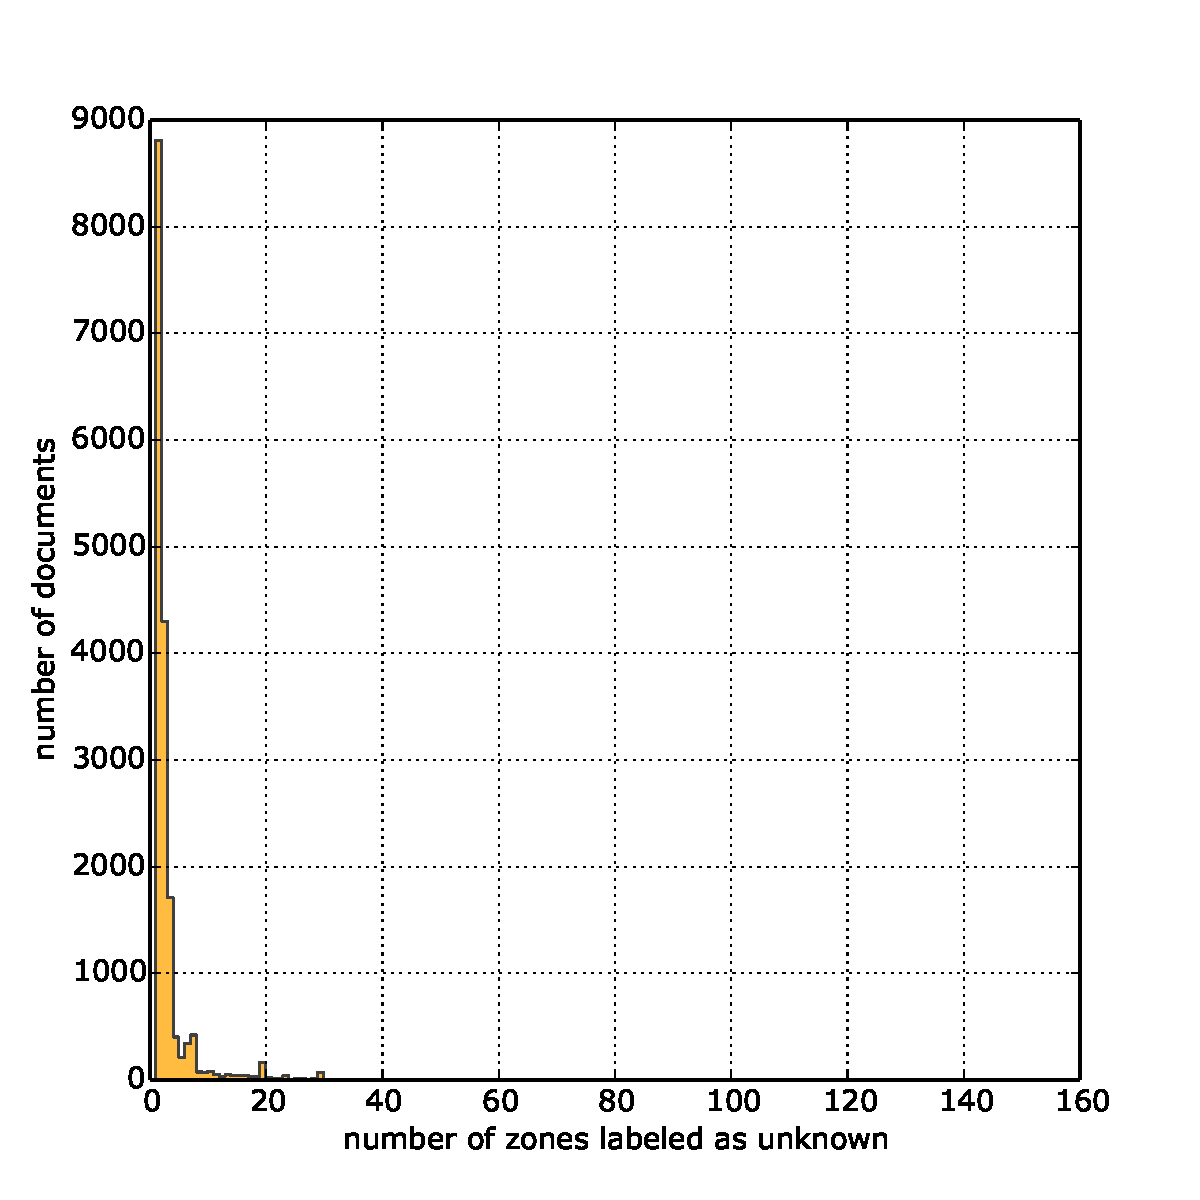
\includegraphics[width=8cm]{plots/unknown_histogram}
  \caption{Histogram of number of zones labeled as \texttt{unknown}}
  \label{fig:unknown_histogram}
\end{minipage}
\end{figure}

\end{appendix}